\documentclass[11pt,a4paper]{article}

\usepackage[a4paper,margin=1in]{geometry}
\usepackage{fontspec}
\usepackage{graphicx}
\usepackage{booktabs}
\usepackage{tabularx}
\usepackage{array}
\usepackage{multirow}
\usepackage{float}
\usepackage{caption}
\usepackage{subcaption}
\usepackage{xcolor}
\usepackage{hyperref}
\usepackage{enumitem}
\usepackage{amsmath}
\usepackage{fancyhdr}
\usepackage{longtable}
\usepackage{microtype}

\setmainfont[
  Path = ../,
  UprightFont = Sarabun.ttf,
  BoldFont = Sarabun.ttf,
  ItalicFont = Sarabun.ttf,
  BoldItalicFont = Sarabun.ttf
]{Sarabun}
\XeTeXlinebreaklocale "th"
\XeTeXlinebreakskip = 0pt plus 1pt

\hypersetup{
  colorlinks=true,
  linkcolor=blue!50!black,
  citecolor=blue!50!black,
  urlcolor=blue!50!black,
  pdftitle={Thai Typing Time-Series Mining Final Report},
  pdfauthor={Thai Typing Time-Series Mining Project}
}

\setlength{\parindent}{0pt}
\setlength{\parskip}{0.55em}
\setlength{\headheight}{14pt}
\setlist[itemize]{leftmargin=1.4em,itemsep=0.2em,topsep=0.2em}
\setlist[enumerate]{leftmargin=1.6em,itemsep=0.2em,topsep=0.2em}
\emergencystretch=3em

\pagestyle{fancy}
\fancyhf{}
\lhead{Thai Typing Time-Series Mining}
\rhead{\thepage}
\renewcommand{\headrulewidth}{0.4pt}

\newcommand{\metric}[1]{\texttt{#1}}
\newcommand{\prompt}[1]{\textbf{#1}}
\newcolumntype{Y}{>{\raggedright\arraybackslash}X}

\title{\vspace{-1.5em}\textbf{Thai Typing Time-Series Mining}\\
\large Correction-Driven Sequential Analysis of Browser-Based Thai Prompt Copying}
\author{
Final Project Report for 2110430 Time Series Mining\\[0.8em]
\begin{tabular}{ll}
6633021421 & Kampanat Yingseree\\
6633232521 & Weerawat Wongmanit\\
6633284121 & Asiwish Chutanunta\\
6642017826 & Jirayu Liangsupong
\end{tabular}\\[0.8em]
\small
Project repository: \href{https://github.com/Kongfha/Typing-Behavior-Time-Series-Analysis}{\texttt{github.com/Kongfha/Typing-Behavior-Time-Series-Analysis}}\\
Study website repository: \href{https://github.com/Kongfha/Thai-Typing-Behavior-Study}{\texttt{github.com/Kongfha/Thai-Typing-Behavior-Study}}
}
\date{April 24, 2026}

\begin{document}
\maketitle

\begin{abstract}
This project studies Thai prompt-copying as a correction-driven time series. A browser task records timestamped edit events while participants copy 14 main prompts containing familiar Thai text, formal language, named entities, numerals, punctuation, and long mixed-difficulty passages. The raw edit stream is reconstructed into aligned event and prompt-position sequences, augmented with Thai Kedmanee keyboard-demand metadata, and analyzed with descriptive statistics, Euclidean baselines, Dynamic Time Warping (DTW), hierarchical clustering, and Matrix Profile discord/motif discovery. After quality control, the main analysis uses 364 main trials from 26 participants. The strongest findings are that Thai numerals, layout-switch punctuation, and selected formal/named-entity spans create shared difficulty, Matrix Profile discords localize these regions on the long prompts, and recovery behavior shows interpretable user-level tendencies when summarized through error episodes and DTW windows.
\end{abstract}

\clearpage
\tableofcontents
\clearpage

\section{Problem Definition}

The project asks whether constrained browser edit logs can reveal meaningful time-series structure in Thai typing behavior. Each trial is a prompt-copying sequence. At each input event, the typed text can be reconstructed and aligned to the target prompt, giving a structured state:

\[
\text{current text} = \text{correct prefix} + \text{wrong suffix}.
\]

This representation turns ordinary browser text-diff logs into a time-series mining problem. The analysis focuses on four research questions:

\begin{enumerate}
  \item \textbf{RQ1: Character- and keyboard-demand fluency.} Which character classes and keyboard conditions are slow or error-prone?
  \item \textbf{RQ2: Linguistic friction and keyboard friction.} How do formal wording, named entities, numerals, punctuation, shift, layout switching, and key distance relate to difficulty?
  \item \textbf{RQ3: Shared difficulty regions.} Do multiple users struggle at the same character spans within a prompt?
  \item \textbf{RQ4: Recovery style.} Do users show different correction patterns after mistakes?
\end{enumerate}

The project is exploratory and interpretation-centered. Its contribution is the transformation of edit-event logs into interpretable time-series objects and the use of course techniques to compare, cluster, and localize behavior.

\section{Dataset and Task Design}

The data come from a browser prompt-copying task. Participants typed one practice prompt followed by 14 main prompts. The prompts were designed to contrast familiar Thai text, formal register, named entities, mixed symbols, Arabic numerals, Thai numerals, rhythmic repetition, and long passages.

\begin{figure}[H]
  \centering
  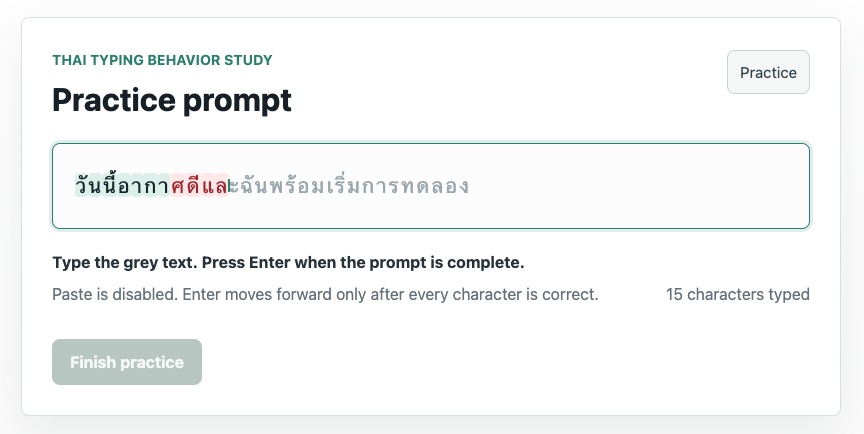
\includegraphics[width=0.78\linewidth]{assets/website_task_screenshot.png}
  \caption{Browser typing task interface used for data collection.}
  \label{fig:website}
\end{figure}

\begin{table}[H]
\centering
\caption{Quality-control scope used for the final analysis.}
\label{tab:qc}
\begin{tabular}{l r}
\toprule
Quantity & Value \\
\midrule
Participants / sessions & 26 \\
Total trials available & 390 \\
Main trials retained for analysis & 364 \\
Practice or warmup trials excluded from main analysis & 26 \\
Main trials failing core QC & 0 \\
Exact-match rate, all trials & 100\% \\
Core QC pass rate, all trials & 100\% \\
\bottomrule
\end{tabular}
\end{table}

\begin{table}[H]
\centering
\caption{Selected prompt-level outcomes after QC.}
\label{tab:prompt_summary}
\small
\begin{tabularx}{\linewidth}{l Y r r r r}
\toprule
Prompt & Condition & Length & Mean duration (s) & Mean deletes & Mean error episodes \\
\midrule
P01 & familiar baseline & 28 & 16.4 & 4.7 & 2.9 \\
P10 & Thai numerals & 46 & 48.2 & 9.7 & 6.1 \\
P12 & long familiar expository & 127 & 54.0 & 16.0 & 7.4 \\
P13 & long formal bureaucratic & 143 & 65.5 & 21.1 & 11.3 \\
P14 & long mixed difficulty & 145 & 69.0 & 18.7 & 10.7 \\
\bottomrule
\end{tabularx}
\end{table}

P10 is short relative to P12-P14 but has the largest duration per character among the highlighted prompts. This makes Thai numerals one of the most visible difficulty mechanisms before any sequence mining is applied.

\section{Methodology Overview}

\subsection{Transformation Pipeline}

The transformation pipeline keeps event-level, position-level, trial-level, and participant-level tables instead of collapsing behavior into a single speed or accuracy score.

\begin{figure}[H]
  \centering
  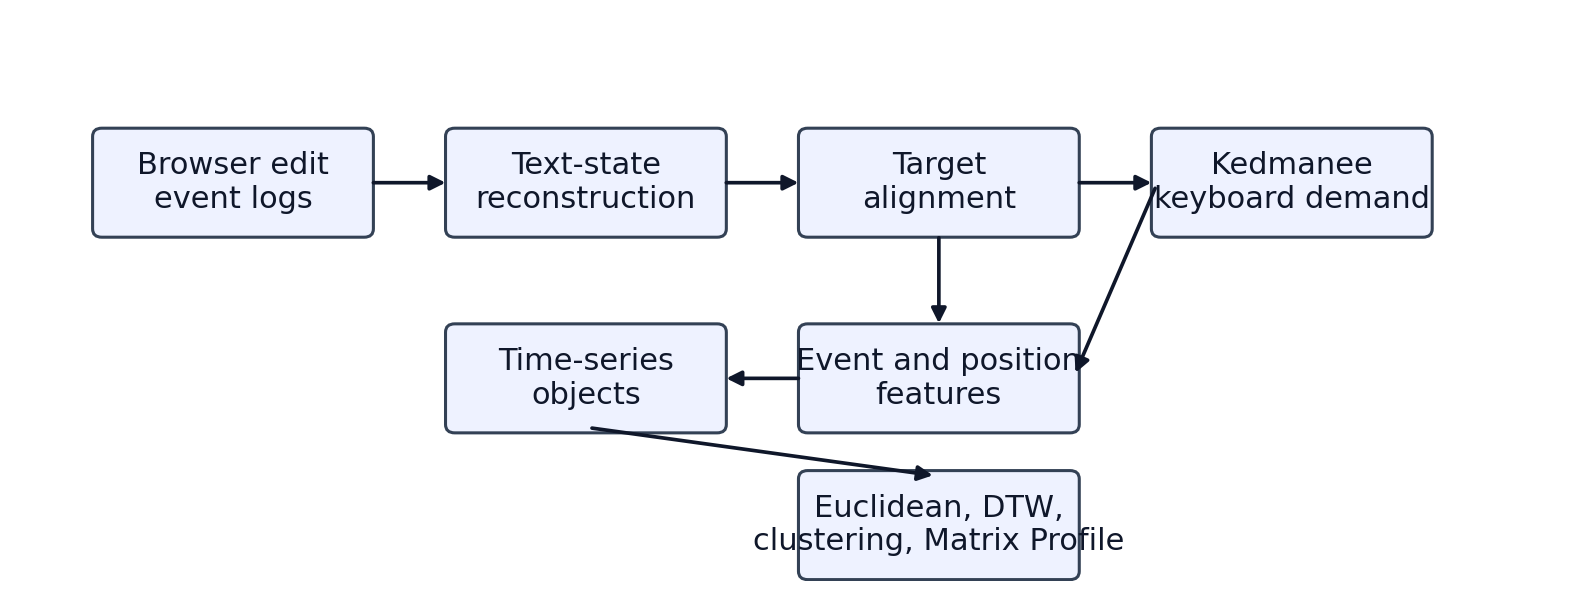
\includegraphics[width=0.82\linewidth]{assets/analysis_pipeline.png}
  \caption{Analysis pipeline from raw browser logs to time-series mining objects.}
  \label{fig:pipeline}
\end{figure}

For every event, the notebook reconstructs \metric{text\_before} and \metric{text\_after}, computes prefix alignment to the target prompt, derives timing and correction features, attaches keyboard metadata, and computes a scalar friction signal:

\begin{align*}
f_t ={}&
0.30z(\log(1+\Delta t_t))
+ 0.25 I(\text{delete}_t) \\
&+ 0.30z(\text{error suffix}_t)
+ 0.08z(\text{planned geometry}_t)
+ 0.02 I(\text{layout switch}_t).
\end{align*}

Here $z(\cdot)$ denotes z-score normalization computed across all events in the dataset; $\Delta t_t$ is the inter-event gap in milliseconds; $I(\cdot)$ is an indicator function; \emph{error suffix} is the number of wrong characters currently at the end of the typed text; and \emph{planned geometry} is the shortest key-graph distance from the previous key to the intended next key. Weights were chosen to give roughly equal importance to timing, correction effort, and error depth, with a small bonus for structural keyboard demand. The resulting scalar rises during struggle (slow keypresses, backspaces, growing wrong suffix) and falls during fluent typing.

The final analysis uses four linked time-series objects:

\begin{table}[H]
\centering
\caption{Main time-series objects.}
\label{tab:objects}
\small
\begin{tabularx}{\linewidth}{l Y Y}
\toprule
Object & Representation & Main use \\
\midrule
A & Event-aligned multivariate sequence: log gap, delete flag, prefix gain, wrong-suffix length, planned geometry burden, layout switch & DTW and recovery comparison \\
B & Scalar friction waveform & Euclidean baseline, DTW baseline, Matrix Profile on long prompts \\
C & Prompt-position stability sequence: time to stability, first-correct time, revisions, wrong-first & Shared difficulty localization \\
D & Participant keyboard-demand profile & Participant comparison and clustering \\
\bottomrule
\end{tabularx}
\end{table}

\subsection{Keyboard-Demand Representation}

Thai keyboard burden is represented through a character map and a graph-distance matrix over physical keys. The distance between two keys is the shortest number of adjacent-key hops on the keyboard graph. This gives an interpretable structural proxy for planned key transition burden and realized mistype proximity. A \emph{layout switch} occurs when consecutive characters in the target prompt belong to different keyboard layers. For example, when a Thai consonant is immediately followed by an Arabic digit or an English punctuation mark. Because the Thai Kedmanee layout is activated by a toggle key (not a modifier held down), the typist must mentally switch context as well as physically change layers, creating a compound burden that is absent within a single layout.

\begin{figure}[H]
  \centering
  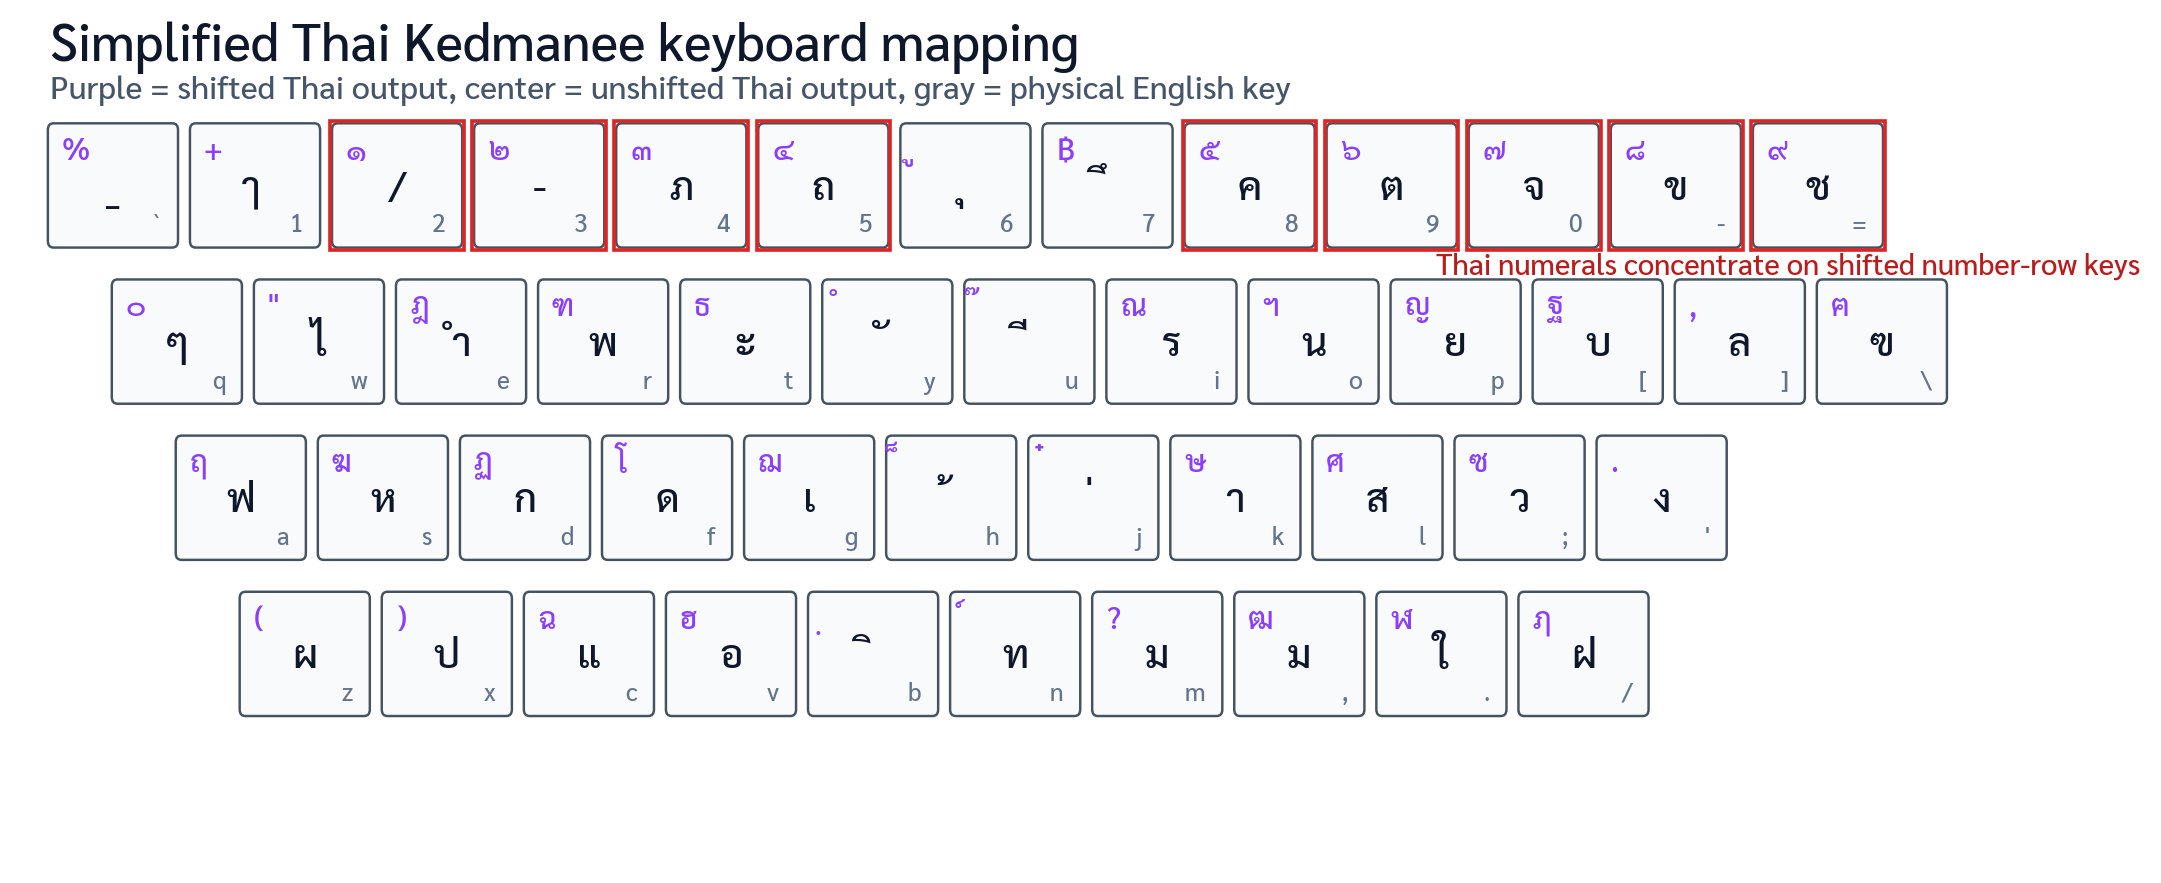
\includegraphics[width=0.98\linewidth]{assets/kedmanee_layout.png}
  \caption{Simplified Thai Kedmanee layout used to explain character-to-key mapping and Thai numeral concentration.}
  \label{fig:kedmanee}
\end{figure}

The keyboard graph connects each key to its surrounding neighbors. The all-pairs shortest-path matrix supplies three core feature columns: \metric{target\_key\_distance}, \metric{layout\_switch\_needed}, and \metric{error\_to\_target\_distance}. Shift requirement and layout requirement are stored as explicit categorical/binary features.

\subsection{Mining and Modeling Methods}

Euclidean distance is used where fixed-length, lockstep comparison is meaningful: participant profiles, same-prompt prompt-position curves, and resampled scalar waveforms. DTW is used for sequences where similar correction behavior may occur at different event positions or speeds \cite{berndt1994dtw}. Hierarchical clustering summarizes participant and recovery structures from the resulting distance matrices. Matrix Profile is used on long-prompt one-dimensional sequences to identify motifs and discords \cite{yeh2016matrixprofile}, the implementation relies on STUMPY \cite{law2019stumpy}.

\section{Evaluation Design}

The evaluation is matched to the exploratory nature of the project. It checks structural validity, method comparison, region-level agreement with frozen difficult spans, cluster stability, Matrix Profile sensitivity, and uncertainty for RQ2 association models.

\begin{table}[H]
\centering
\caption{Evaluation components and evidence reported.}
\label{tab:evaluation_design}
\small
\begin{tabularx}{\linewidth}{l Y}
\toprule
Component & Evidence \\
\midrule
QC validity & Trial/session inclusion, exact-match reconstruction rate, core QC flags \\
Euclidean vs DTW & Same-prompt retrieval, within/between distance ratio, neighbor overlap \\
Frozen difficult spans & Same-length window ranks and inside-minus-outside friction \\
Clustering & Silhouette, cophenetic correlation, cluster-size balance, linkage sensitivity \\
Matrix Profile & Discord overlap under nearby window sizes and overlap with frozen spans \\
RQ2 models & Coefficients, participant-clustered confidence intervals, fit statistics \\
\bottomrule
\end{tabularx}
\end{table}

\section{Results}

\subsection{RQ1: Character- and Keyboard-Demand Fluency}

\begin{figure}[H]
  \centering
  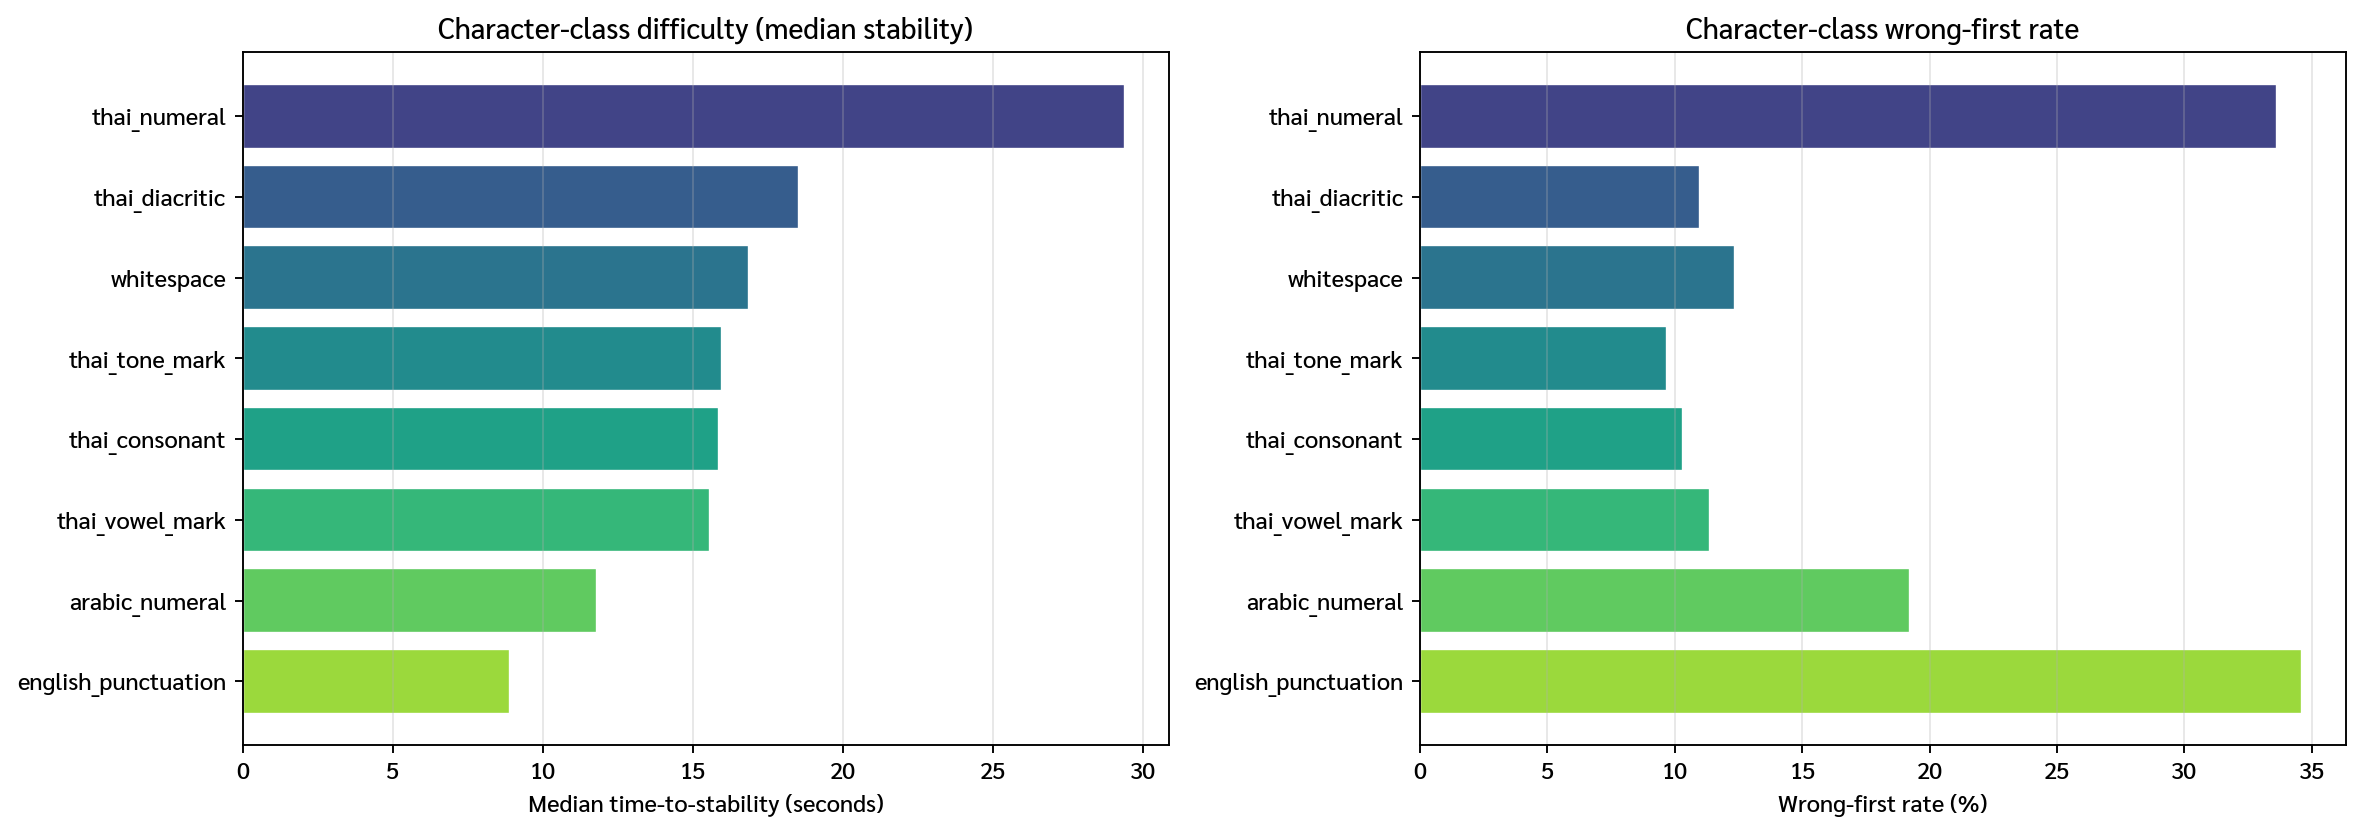
\includegraphics[width=0.96\linewidth]{assets/character_class_difficulty.png}
  \caption{Character-class difficulty by stability time and wrong-first rate.}
  \label{fig:charclass}
\end{figure}

\begin{table}[H]
\centering
\caption{Character-class difficulty summary.}
\label{tab:char_class}
\small
\begin{tabular}{l r r r}
\toprule
Character class & Positions & Median stability (s) & Wrong-first rate \\
\midrule
Thai numeral & 104 & 29.4 & 33.7\% \\
Thai diacritic & 182 & 18.5 & 11.0\% \\
Whitespace & 494 & 16.9 & 12.3\% \\
Thai tone mark & 1,404 & 16.0 & 9.7\% \\
Thai consonant & 13,520 & 15.9 & 10.3\% \\
Thai vowel mark & 6,162 & 15.6 & 11.4\% \\
Arabic numeral & 130 & 11.8 & 19.2\% \\
English punctuation & 78 & 8.9 & 34.6\% \\
\bottomrule
\end{tabular}
\end{table}

Thai numerals are the most difficult class on both timing and first-attempt accuracy. English punctuation has a different signature: participants often commit quickly, but wrong-first rate is the highest class-level value. Frequent Thai consonants, vowels, and tone marks are much more uniform.

\begin{figure}[H]
  \centering
  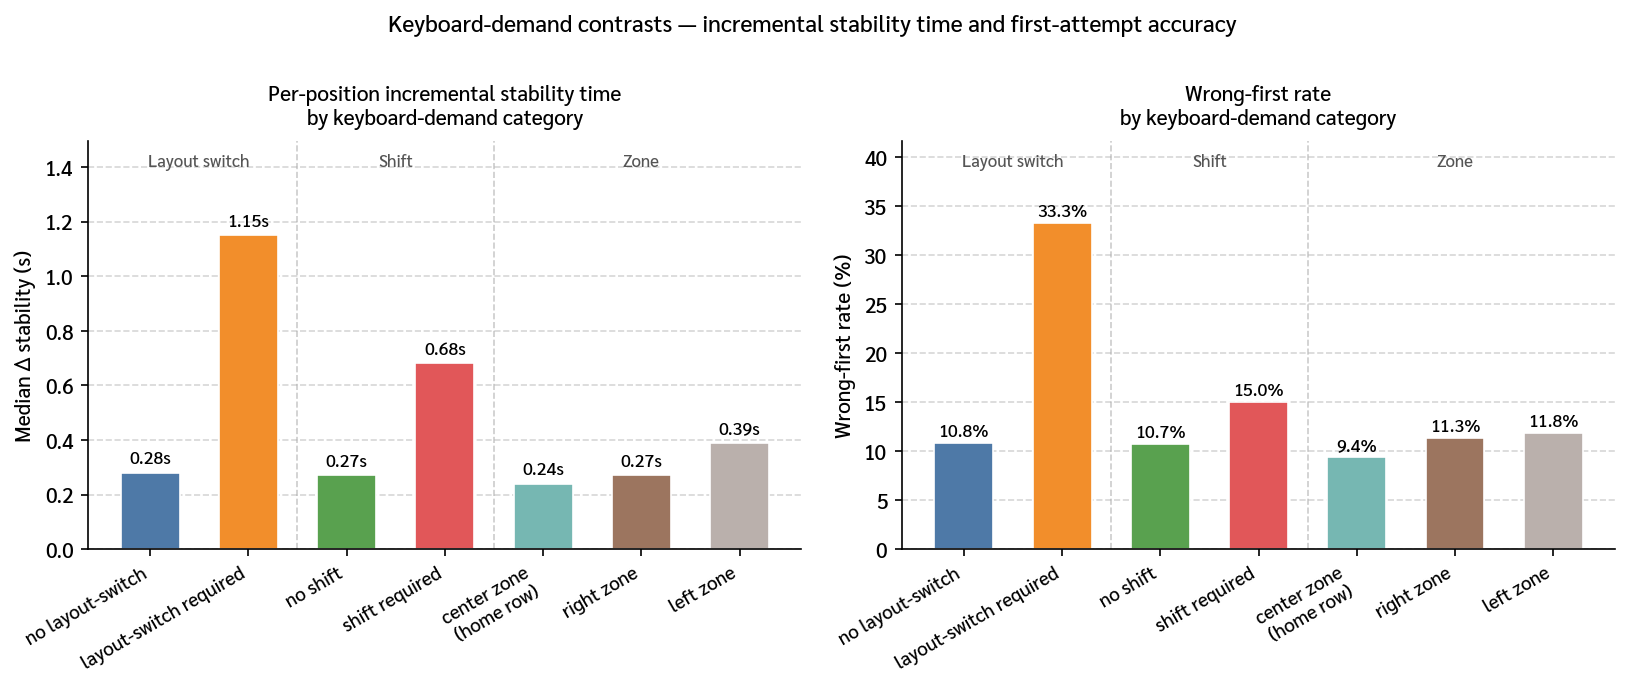
\includegraphics[width=0.96\linewidth]{assets/keyboard_demand_compare.png}
  \caption{Keyboard-demand contrasts by stability time and wrong-first rate.}
  \label{fig:keyboardcompare}
\end{figure}

Keyboard-demand contrasts are measured using the per-position incremental stability time ($\Delta$\,stability), computed as the first difference of \metric{time\_to\_stability\_ms} across consecutive positions within each prompt curve. This isolates the local cost added at each position rather than confounding it with cumulative elapsed time from the start of the prompt.

\begin{table}[H]
\centering
\caption{Keyboard-demand contrasts: per-position incremental stability time and wrong-first rate.}
\label{tab:keyboard_demand}
\small
\begin{tabular}{l r r}
\toprule
Contrast & Median $\Delta$ stability (s) & Wrong-first rate \\
\midrule
No layout-switch       & 0.28 & 10.8\% \\
\textbf{Layout-switch required} & \textbf{1.15} & \textbf{33.3\%} \\
No shift               & 0.27 & 10.7\% \\
Shift required         & 0.68 & 15.0\% \\
Center zone (home row) & 0.24 &  9.4\% \\
Right zone             & 0.27 & 11.3\% \\
Left zone              & 0.39 & 11.8\% \\
\bottomrule
\end{tabular}
\end{table}

Layout-switch positions are the clearest signal on both dimensions: they are approximately four times slower per position (1.15\,s vs 0.28\,s) and three times more likely to produce a wrong first keystroke (33\% vs 11\%). The previous cumulative-time representation obscured this penalty because layout switches tend to occur mid-prompt, where cumulative elapsed time is already large regardless of per-key difficulty. With incremental time, the local cost of switching keyboard layers becomes visible. Shift-required positions show a smaller but consistent penalty (0.68\,s, 15\% wrong-first). The left zone has the highest incremental time among the three zones (0.39\,s), consistent with tone marks and diacritics concentrated on the weaker left-hand fingers in the Thai Kedmanee layout.

\subsection{RQ2: Linguistic Friction and Keyboard Friction}

The association models use prompt-position observations with participant-clustered uncertainty. The clearest timing associations are Thai numerals, prompt-level formal/mixed difficulty, Thai diacritics, and layout switching. The outcome variable is $\log(\text{time\_to\_stability\_ms})$, so a coefficient of $c$ means the predicted log-stability increases by $c$ log-milliseconds relative to the baseline. Equivalently, the expected stability time is multiplied by $e^c$. For example, the Thai-numeral coefficient of 1.578 corresponds to a multiplicative factor of $e^{1.578} \approx 4.8$, meaning a Thai numeral position is predicted to take roughly five times longer to stabilize than a baseline Thai consonant in the same prompt.

\begin{table}[H]
\centering
\caption{Selected RQ2 associations for log time-to-stability.}
\label{tab:rq2_coeff}
\small
\begin{tabularx}{\linewidth}{l r r r Y}
\toprule
Term & Coef. & 95\% CI low & 95\% CI high & Interpretation \\
\midrule
Thai numeral class & 1.578 & 1.413 & 1.743 & Largest character-class timing penalty \\
Prompt P14 fixed effect & 1.577 & 1.399 & 1.755 & Mixed long prompt effect \\
Prompt P13 fixed effect & 1.508 & 1.352 & 1.665 & Formal bureaucratic prompt effect \\
Thai diacritic class & 0.696 & 0.635 & 0.756 & Rare mark burden \\
Layout switch into position & 0.321 & 0.290 & 0.351 & Keyboard-state burden \\
Physical key distance & 0.0177 & 0.0160 & 0.0193 & Small per-hop increase \\
\bottomrule
\end{tabularx}
\end{table}

The RQ2 result is additive rather than either/or. Per-character keyboard effects are strongest at Thai numerals, diacritics, and layout-switch positions. Prompt-level effects are strongest for long formal and mixed-difficulty prompts. P14 combines both: a Thai numeral appears inside a formal educational phrase, and that span becomes one of the strongest local difficulty regions.

\subsection{RQ3: Shared Difficulty Regions}

\begin{figure}[H]
  \centering
  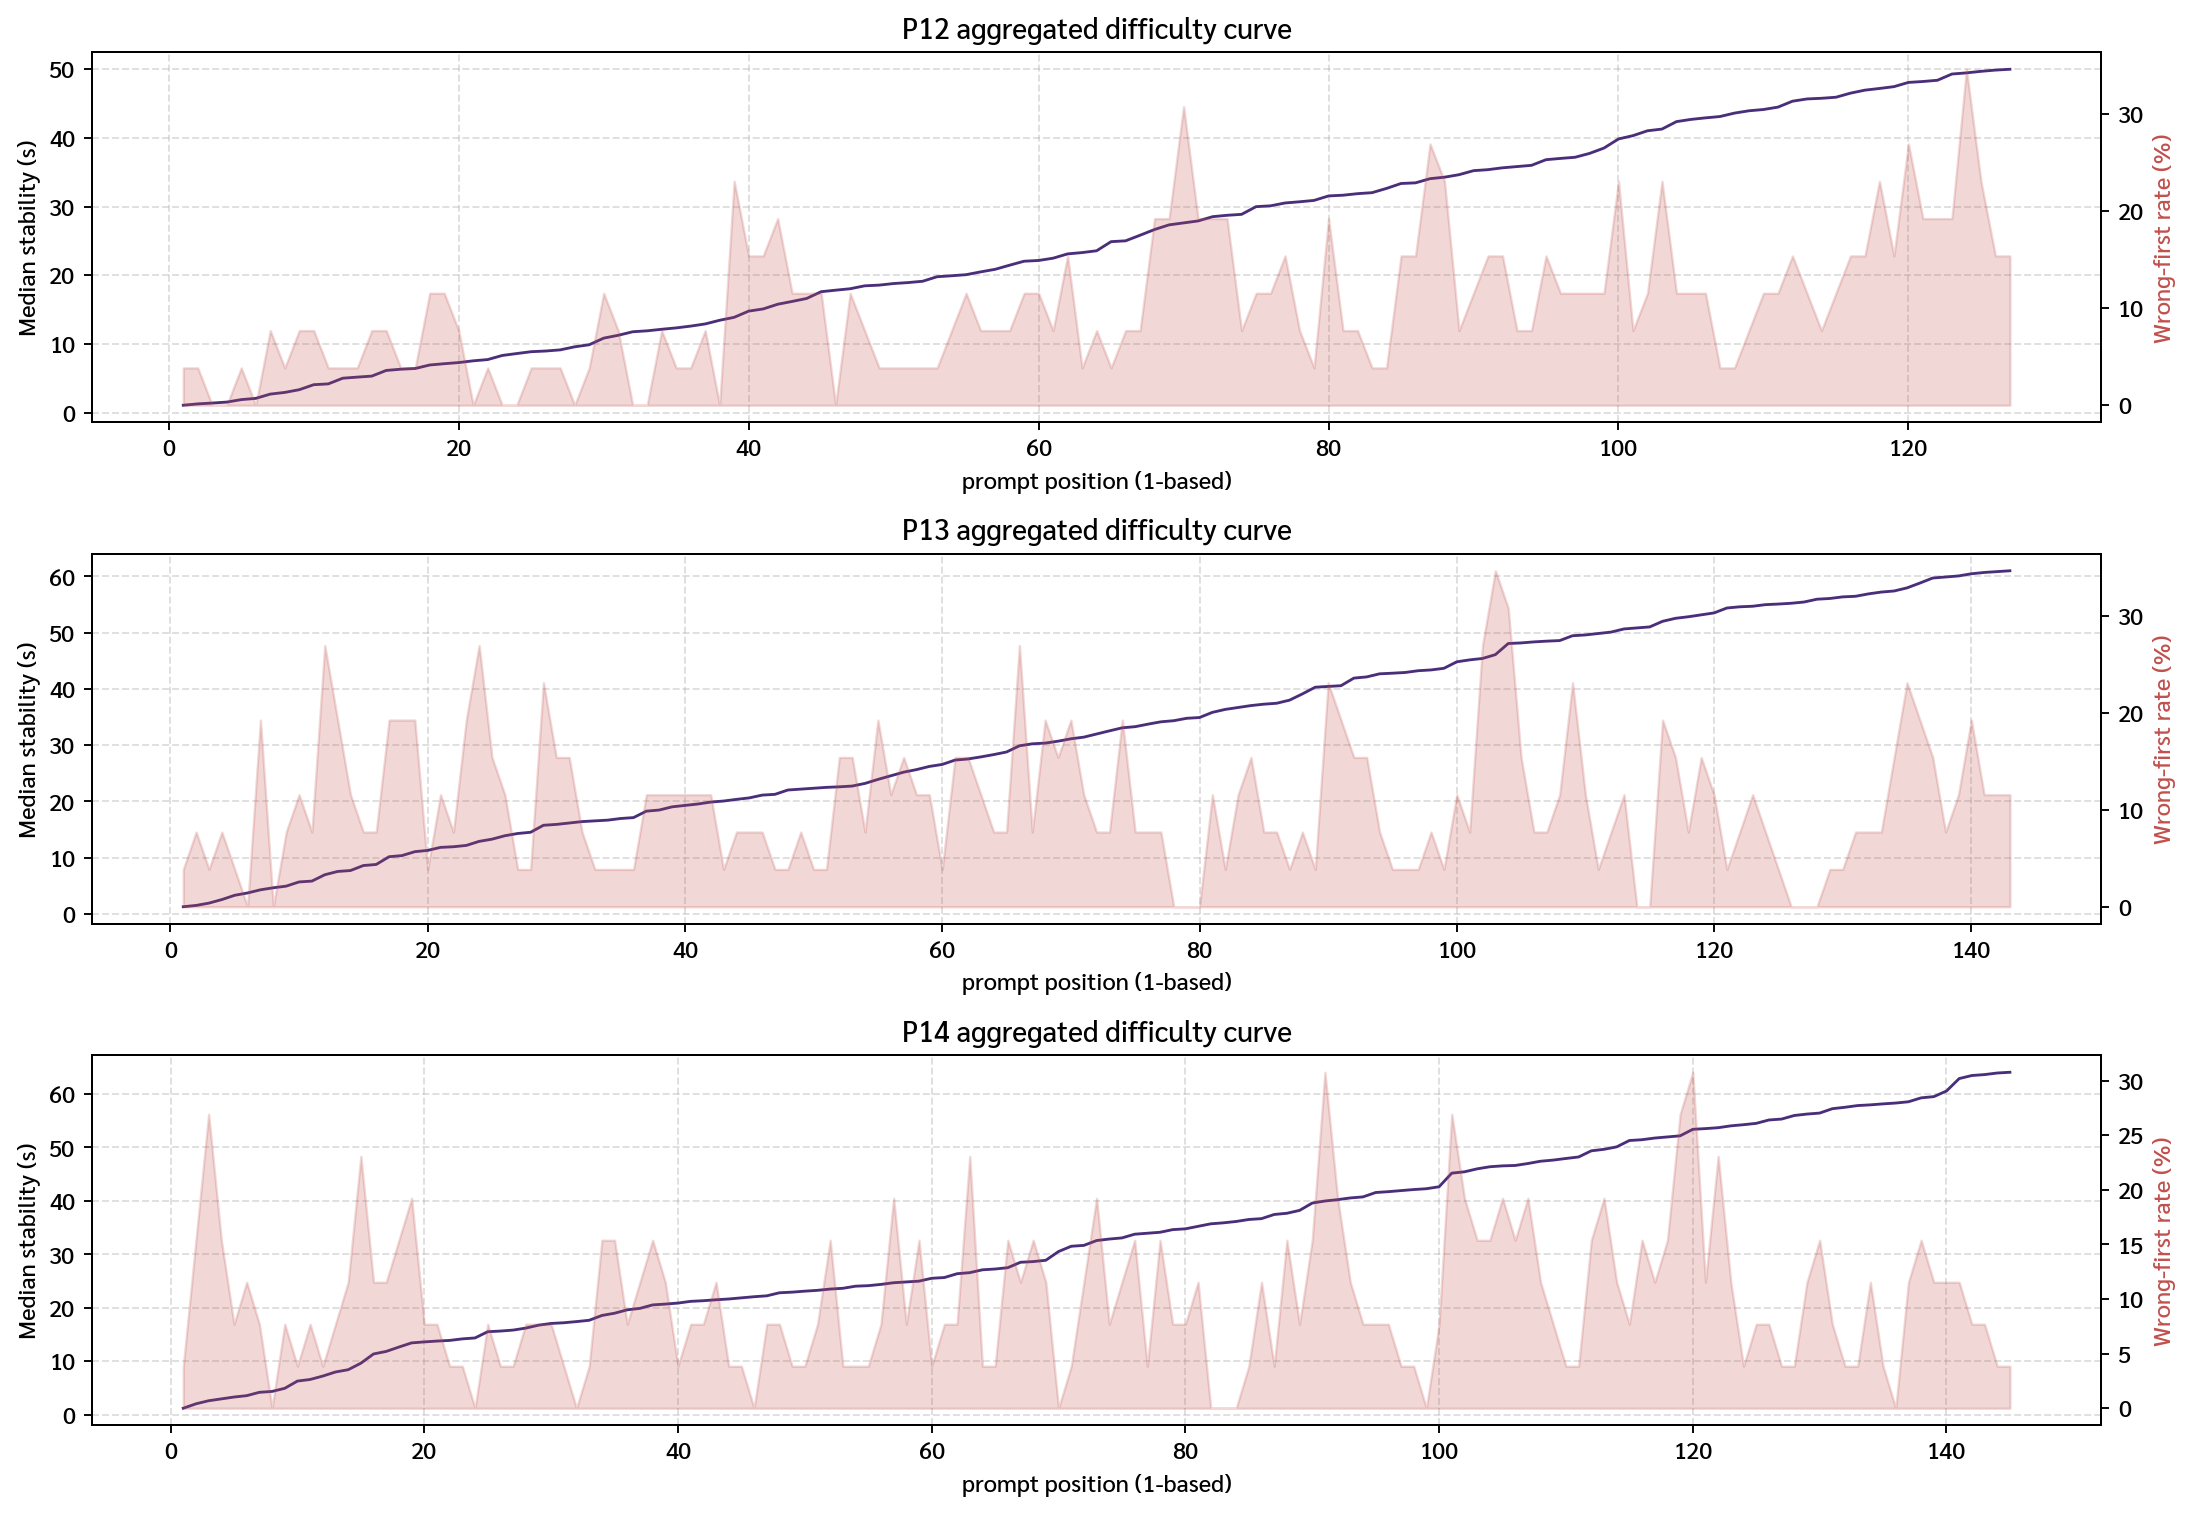
\includegraphics[width=0.95\linewidth]{assets/long_prompt_aggregated_difficulty_curves.png}
  \caption{Aggregated difficulty curves for P12, P13, and P14.}
  \label{fig:longcurves}
\end{figure}

Shared difficulty is most visible on the long prompts. Aggregated curves, local peaks, same-prompt distance heatmaps, and Matrix Profile discords point to compact spans rather than entire prompts. In the Matrix Profile framework, a \emph{discord} is a subsequence whose nearest neighbor in the same time series is farther away than any other subsequence's nearest neighbor, in other words, it is the most ``unusual'' shape in the curve. Applied to the aggregated difficulty curve of a prompt, a high-MP-distance discord identifies a span of positions where the joint difficulty profile (stability time and wrong-first rate together) is unlike anything else in that prompt. A \emph{motif}, by contrast, is the most frequently repeating shape, typically a baseline fluent region. High MP distance therefore serves as an unsupervised flag for locally anomalous difficulty without requiring any manual labeling of hard spans.

\begin{figure}[H]
  \centering
  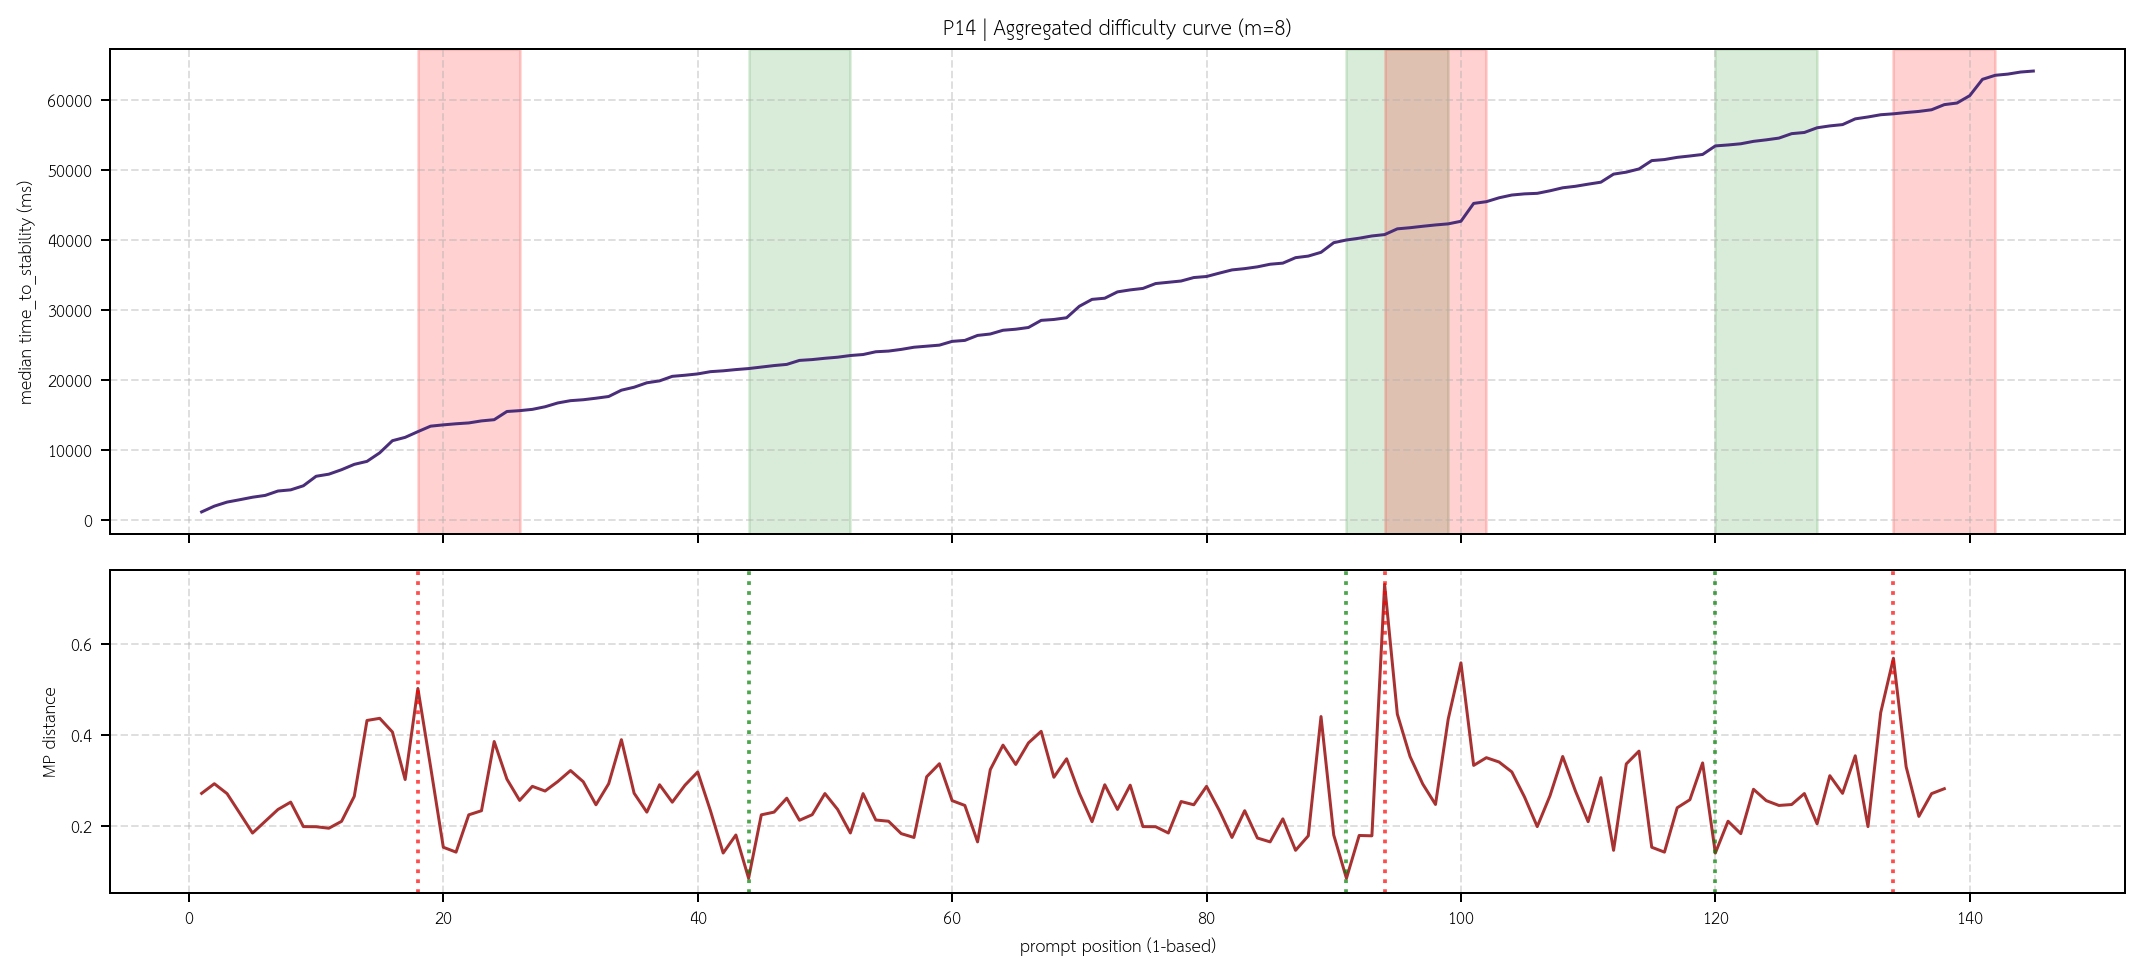
\includegraphics[width=0.90\linewidth]{assets/mp_aggregated_curve_P14.png}
  \caption{Matrix Profile on the P14 aggregated prompt-position curve. The top discord covers the Thai numeral span around ``ปีที่ ๖''.}
  \label{fig:p14mp}
\end{figure}

\begin{table}[H]
\centering
\caption{Top Matrix Profile discord spans on aggregated long-prompt curves.}
\label{tab:mp_spans}
\small
\begin{tabular}{l l r r l}
\toprule
Prompt & Span & Positions & MP distance & Dominant interpretation \\
\midrule
P14 & าปีที่ ๖ & 94-101 & 0.730 & Thai numeral inside formal phrase \\
P14 & ครือพันธ & 134-141 & 0.568 & Named-entity region \\
P13 & นเพื่อเป & 103-110 & 0.604 & Formal connective boundary \\
P13 & ายเนื้อห & 85-92 & 0.409 & Formal noun phrase \\
P12 & รุปเรื่อ & 29-36 & 0.390 & Distributed expository difficulty \\
\bottomrule
\end{tabular}
\end{table}

The frozen-span evaluation supports the same interpretation. Several predefined spans rank near the top among same-length windows for friction, including P04 จุฬาลงกรณ์, P10 ๑๐, P06 ม.5/6, P14 ชาคริษฐ์, and P14 ๖. Positive inside-minus-outside friction appears for all ten evaluated spans.

\begin{table}[H]
\centering
\caption{Selected frozen-span validation results. Rank 1 is the highest same-length window in the prompt.}
\label{tab:frozen}
\small
\begin{tabularx}{\linewidth}{l l Y r r r}
\toprule
Prompt & Span & Mechanism & Friction rank & Windows & Inside-minus-outside friction \\
\midrule
P04 & จุฬาลงกรณ์ & named entity & 1 & 20 & 0.123 \\
P10 & ๑๐ & Thai numeral & 1 & 45 & 0.609 \\
P06 & ม.5/6 & mixed symbols & 3 & 48 & 0.262 \\
P14 & ชาคริษฐ์ & named entity & 1 & 138 & 0.232 \\
P14 & ๖ & Thai numeral & 5 & 143 & 0.312 \\
P13 & สุภาษิต & formal vocabulary & 14 & 137 & 0.124 \\
\bottomrule
\end{tabularx}
\end{table}

\subsection{RQ4: Recovery Style}

The analysis identifies 1,787 error episodes after QC. A rule-based recovery summary gives a compact view of how participants correct mistakes.

\begin{table}[H]
\centering
\caption{Recovery episode style counts.}
\label{tab:recovery_counts}
\begin{tabular}{l r r}
\toprule
Recovery style & Episodes & Share \\
\midrule
Other or shallow episode & 1,276 & 71\% \\
Deep overshoot then recovery & 282 & 16\% \\
Immediate repair & 143 & 8\% \\
Pause then delete & 86 & 5\% \\
\bottomrule
\end{tabular}
\end{table}

\begin{figure}[H]
  \centering
  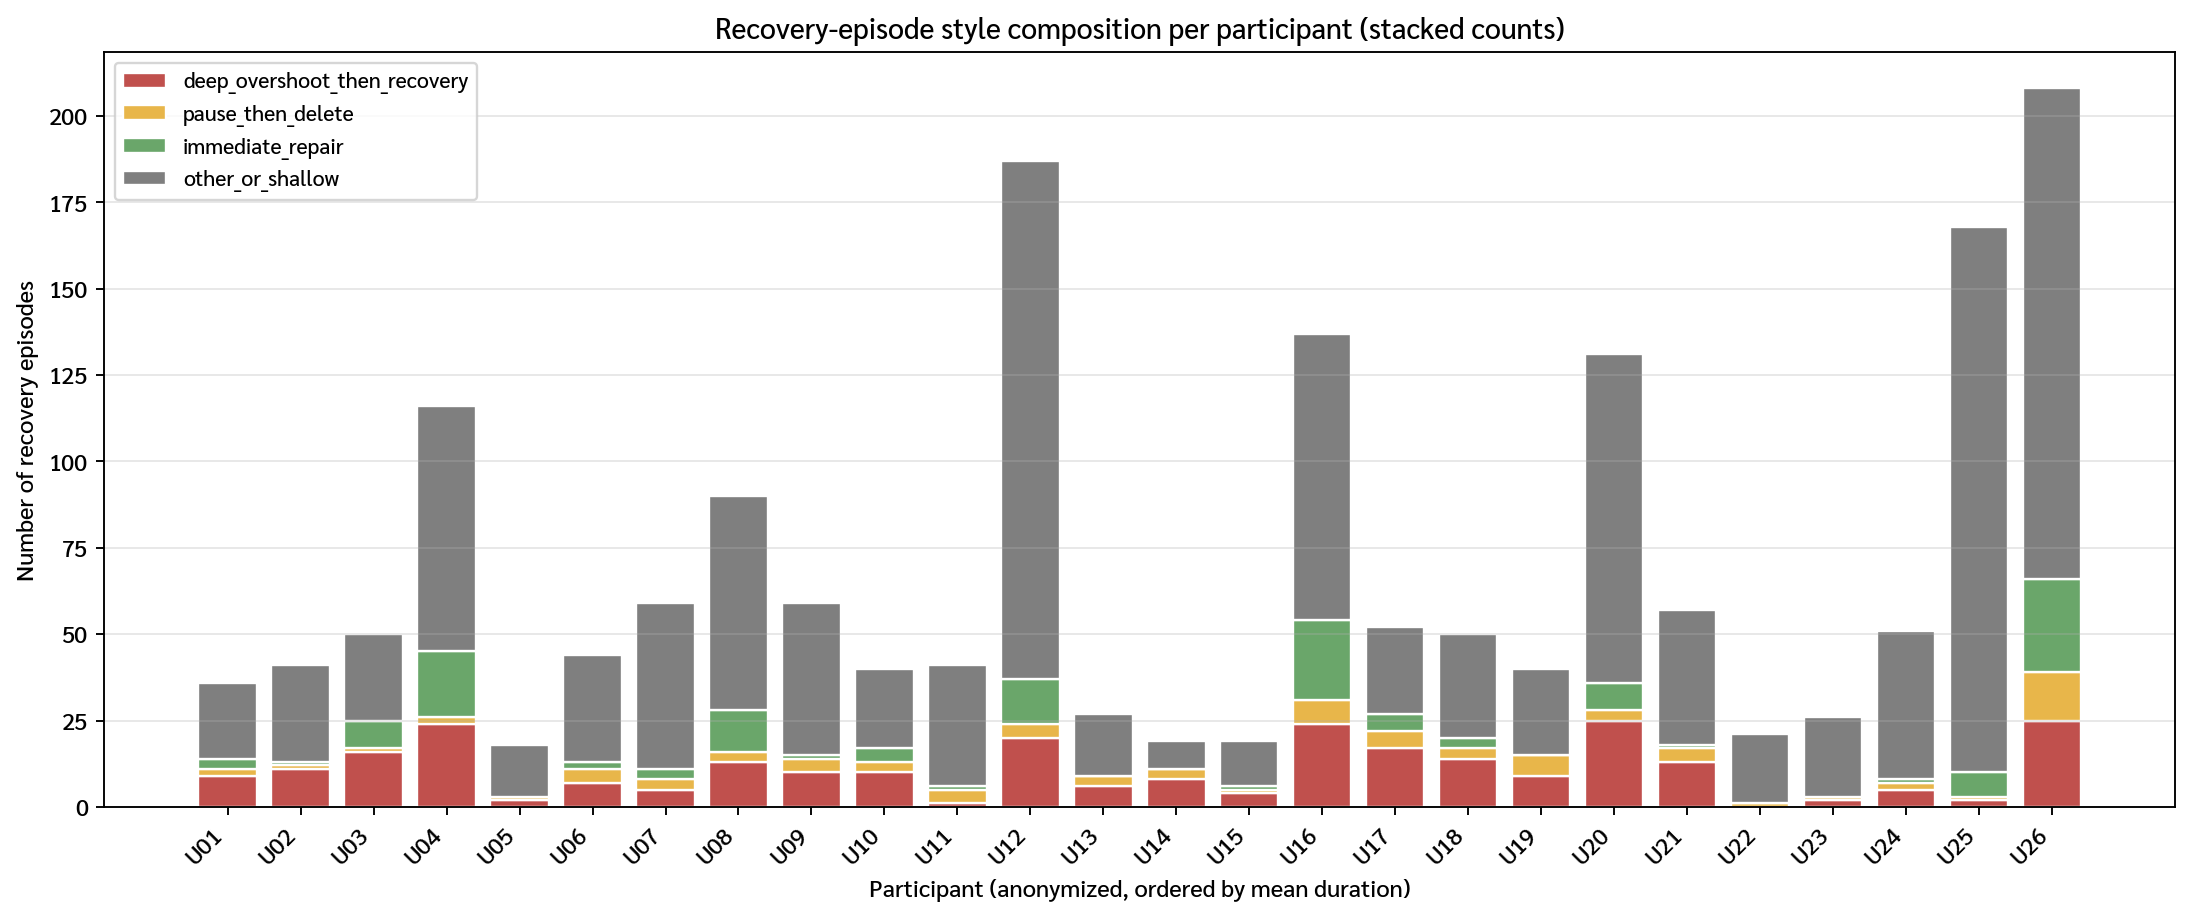
\includegraphics[width=0.95\linewidth]{assets/recovery_style_stacked.png}
  \caption{Per-participant recovery-style composition using anonymized participant IDs.}
  \label{fig:recovery}
\end{figure}

DTW windows around error episodes organize recovery behavior into descriptive groups: immediate repair, pause-then-delete, deep overshoot followed by recovery, and burst-like mixed correction. The cluster diagnostics show that these groups are exploratory, their value is strongest when read together with episode summaries and representative traces.

\begin{figure}[H]
  \centering
  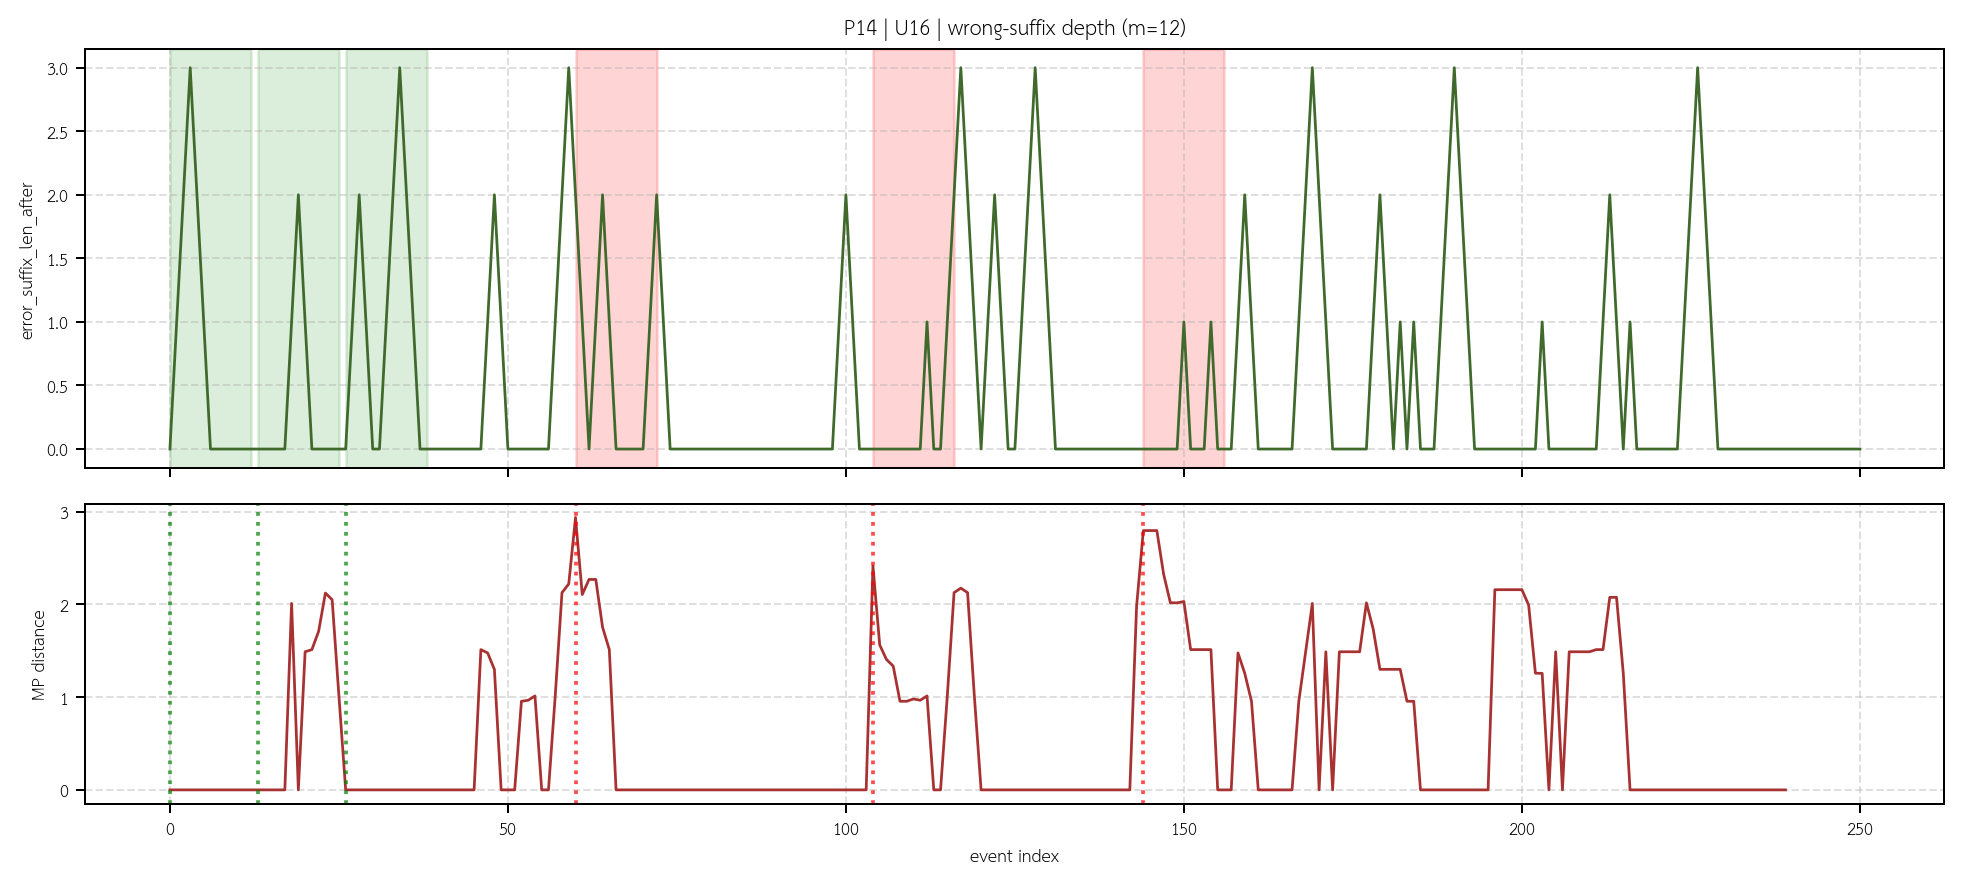
\includegraphics[width=0.90\linewidth]{assets/mp_error_suffix_P14_U16.png}
  \caption{Representative Matrix Profile view of \metric{error\_suffix\_len\_after} for U16 on P14, showing repeated wrong-suffix spikes and a prominent anomalous recovery region.}
  \label{fig:error_suffix_mp}
\end{figure}

\section{Method Comparison and Robustness}

\subsection{Euclidean and DTW Retrieval}

The evaluation compares Euclidean and constrained DTW on the same resampled scalar friction waveform representation. DTW is comparable to Euclidean on this compact waveform object, while its main interpretive value remains recovery-window alignment.

\begin{table}[H]
\centering
\caption{Same-prompt retrieval on resampled friction waveforms.}
\label{tab:euclidean_dtw}
\small
\begin{tabular}{l r r r r}
\toprule
Method & Band & Top-1 & Top-3 & Within/between ratio \\
\midrule
Euclidean & - & 52.7\% & 72.0\% & 0.920 \\
DTW & 0.08 & 54.4\% & 73.6\% & 0.883 \\
DTW & 0.12 & 51.9\% & 72.3\% & 0.889 \\
DTW & 0.16 & 51.4\% & 71.7\% & 0.894 \\
\bottomrule
\end{tabular}
\end{table}

\begin{figure}[H]
  \centering
  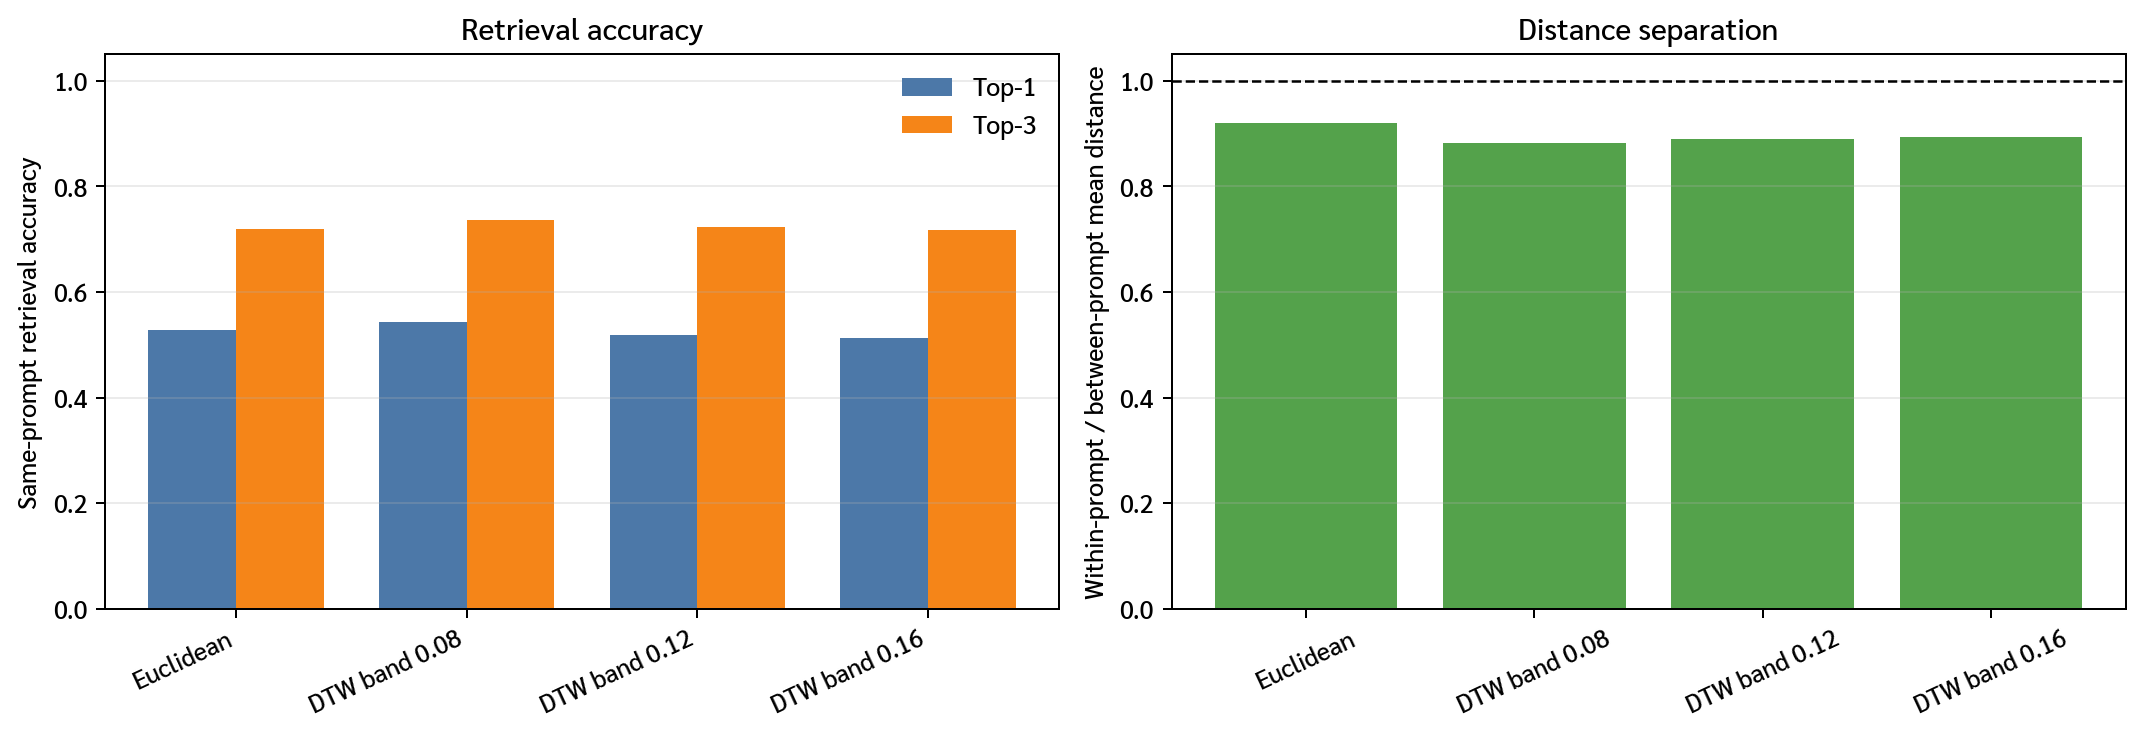
\includegraphics[width=0.85\linewidth]{assets/euclidean_vs_dtw_retrieval_comparison.png}
  \caption{Euclidean-vs-DTW retrieval comparison on the scalar friction waveform object.}
  \label{fig:retrieval}
\end{figure}

\subsection{Clustering and Matrix Profile Stability}

Cluster diagnostics are useful as sanity checks. Participant-profile and prompt-position Euclidean clusters have positive silhouette scores, while DTW cluster objects also show positive but modest distance-based silhouette values. Several cluster solutions are imbalanced, so cluster labels are treated as descriptive summaries rather than fixed classes.

\begin{table}[H]
\centering
\caption{Clustering evaluation summary.}
\label{tab:cluster_eval}
\small
\begin{tabular}{l r r r r}
\toprule
Cluster object & Objects & Clusters & Silhouette & Largest cluster share \\
\midrule
Participant profile, Euclidean & 26 & 3 & 0.226 & 0.923 \\
Prompt-position P14, Euclidean & 26 & 3 & 0.385 & 0.923 \\
Trial-event P13, DTW & 26 & 3 & 0.169 & 0.654 \\
Error episode, DTW & 120 & 4 & 0.237 & 0.917 \\
\bottomrule
\end{tabular}
\end{table}

Matrix Profile sensitivity is strongest for P13 and P14. P14 keeps high overlap between default and nearby window sizes, and the nearby windows continue to overlap the Thai-numeral and named-entity frozen spans.

\begin{figure}[H]
  \centering
  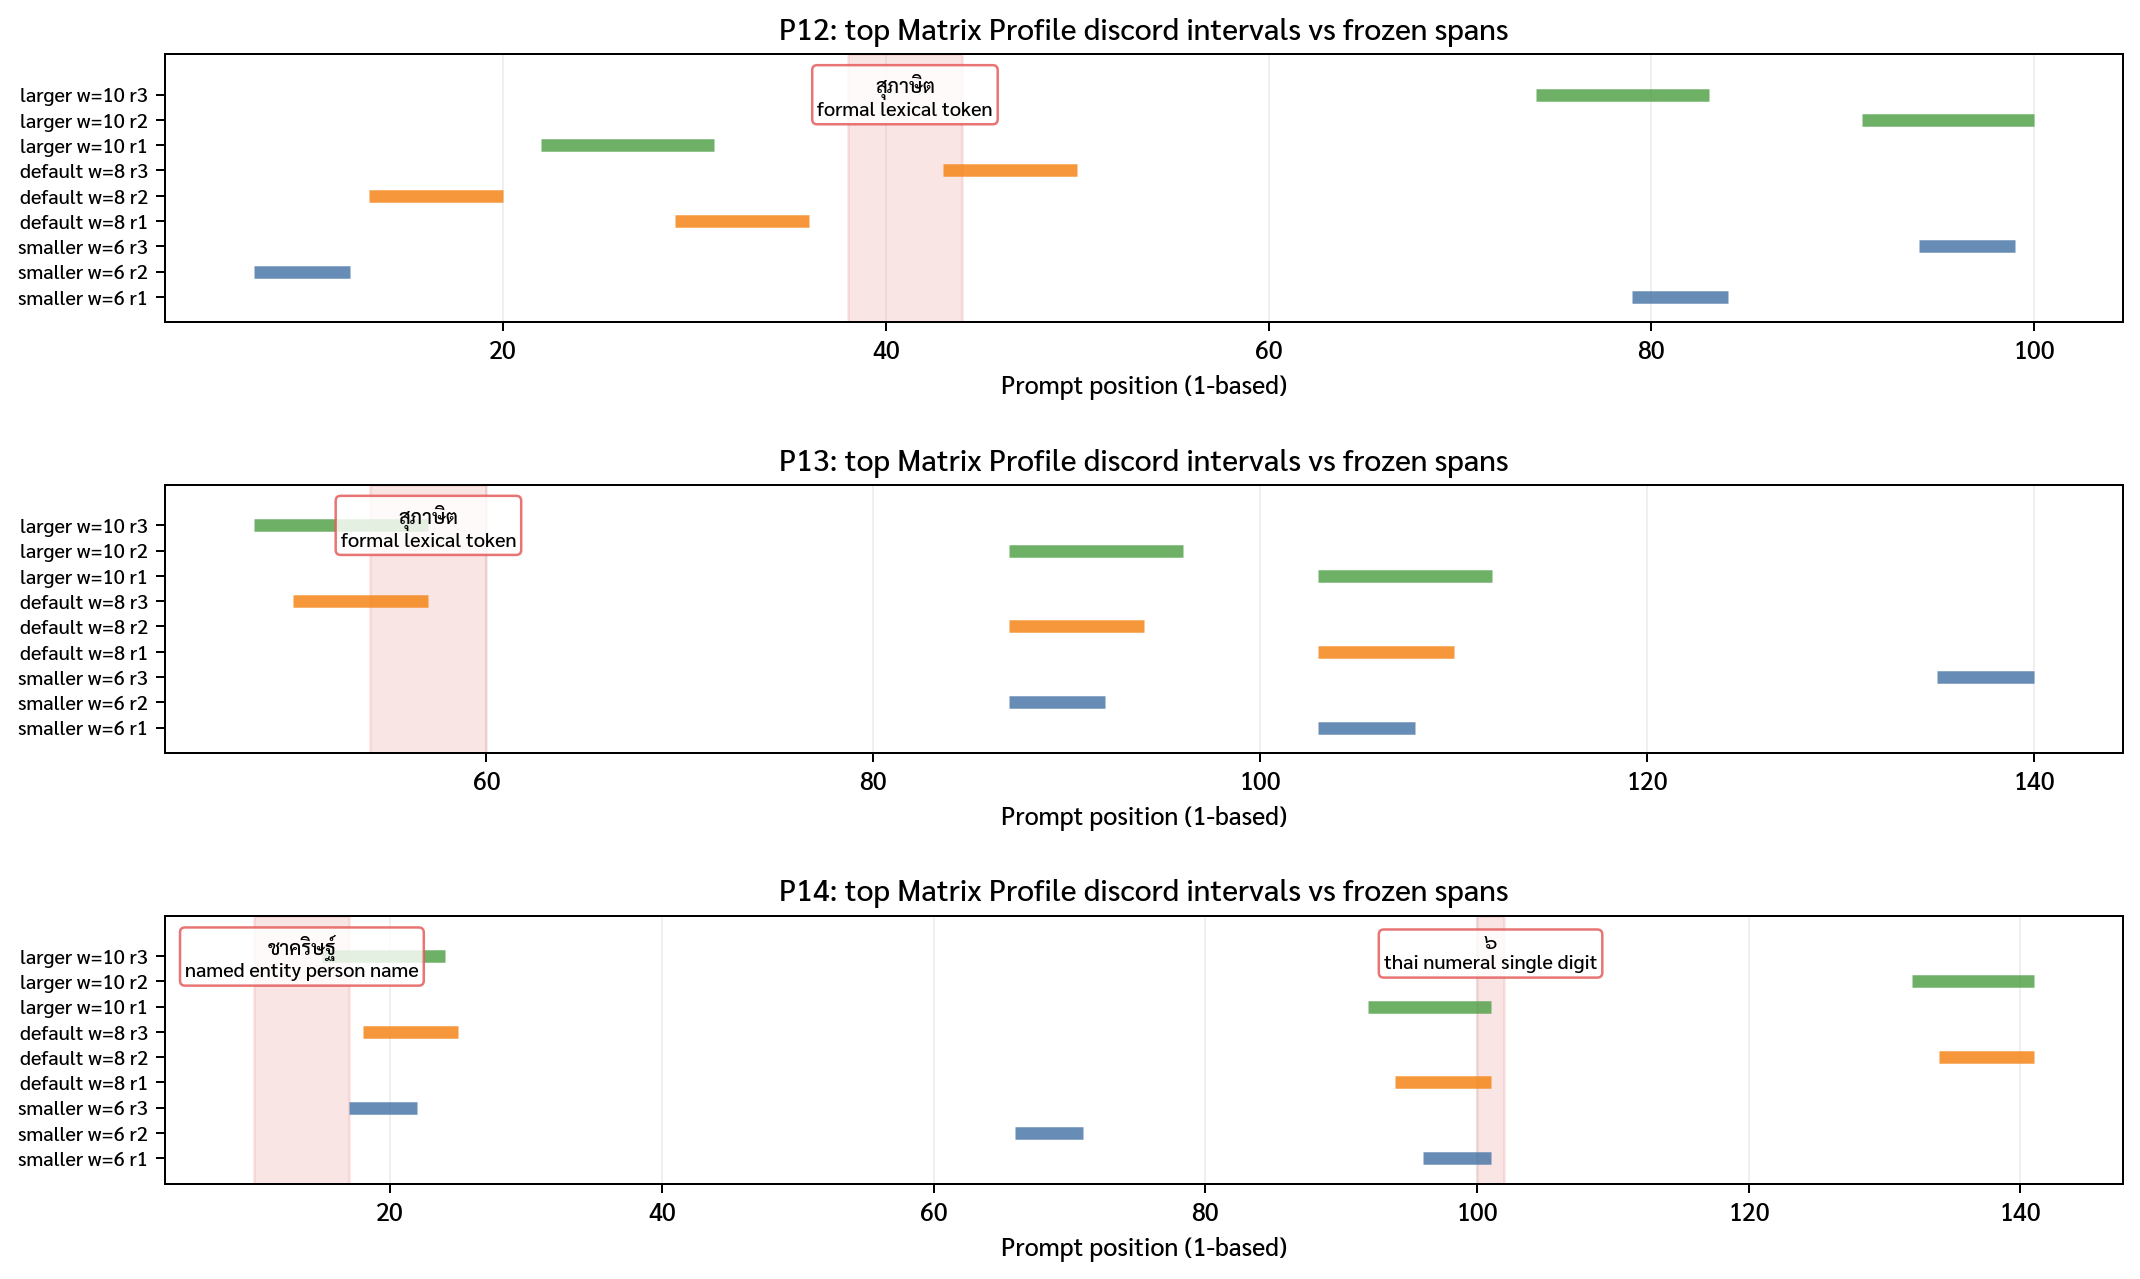
\includegraphics[width=0.82\linewidth]{assets/matrix_profile_sensitivity_overlap.png}
  \caption{Matrix Profile top-discord overlap under nearby window sizes.}
  \label{fig:mp_sensitivity}
\end{figure}

\section{Conclusion}

The project satisfies the final-project goal by turning a self-collected Thai typing dataset into a clear time-series mining pipeline. The strongest evidence comes from agreement across representations: prompt-position metrics, keyboard-demand features, Euclidean and DTW comparisons, Matrix Profile discords, and frozen-span validation all highlight the same mechanisms. Thai numerals are the most consistent keyboard-demand difficulty signal, formal phrases and named entities create localized linguistic friction, and recovery episodes reveal participant-level correction tendencies that are visible beyond simple speed ranking.

The results should be interpreted as exploratory evidence from 26 volunteer sessions. Within that scope, the analysis is technically coherent, interpretable, and aligned with the course emphasis on representation choice, similarity measures, motif/discord discovery, clustering, and critical evaluation.

Several directions could strengthen these findings in future work. Recruiting a larger and more demographically diverse participant pool would help assess whether the cluster imbalance observed here (where a single large cluster dominates participant and prompt-position groupings) reflects a genuine behavioral majority or merely a sampling artifact from a convenience sample of university students. Testing prompts that deliberately vary linguistic friction mechanisms, for example, isolating Thai numerals from named entities, or contrasting formal register with informal text of matched length, would allow a more controlled decomposition of keyboard and linguistic effects than the additive OLS model currently provides. Finally, applying the Matrix Profile analysis to participants' native-language typing data would establish an individual baseline, making it possible to quantify how much of the observed difficulty is specific to Thai script versus a general unfamiliarity with prompt-copying tasks.

\appendix
\clearpage

\section{Prompt Inventory}

The main prompt order and prompt texts used in the final analysis are listed below.

\begin{longtable}{p{0.07\linewidth} p{0.13\linewidth} p{0.24\linewidth} p{0.45\linewidth}}
\caption{Main prompt inventory.}
\label{tab:prompt_inventory}\\
\toprule
ID & Length & Condition & Prompt text \\
\midrule
\endfirsthead
\toprule
ID & Length & Condition & Prompt text \\
\midrule
\endhead
P01 & short & familiar baseline & วันนี้เราจะทำการบ้านให้เสร็จ \\
P02 & short & familiar polite & กรุณาตอบกลับภายในวันนี้ \\
P04 & short & orthographic named entity & นิสิตจากจุฬาลงกรณ์มหาวิทยาลัย \\
P03 & short & formal register & ขอความกรุณาจัดทำเอกสารดังกล่าว \\
P05 & short & twisted proverb & เข้าเมืองตาหลิ่ว ต้องหลิ่วมาตาม \\
P09 & medium & Arabic numerals & ชั้นมัธยมศึกษาปีที่ 6 จะส่งรายงานจำนวน 10 หน้า \\
P11 & medium & rhythmic repetition & วันนี้ผมทักผมรักผมรอ วันไหนผมท้อผมพอผมลา \\
P10 & medium & Thai numerals & ชั้นมัธยมศึกษาปีที่ ๖ จะส่งรายงานจำนวน ๑๐ หน้า \\
P06 & medium & mixed symbols identification & นักเรียน ม.5/6 ช่วยตรวจสอบ ชื่อ-สกุล ของตัวเองด้วยนะ \\
P08 & medium & formal lexical difficulty & ขอความร่วมมือจัดเตรียมเอกสารเพื่อเป็นวิทยาทานแก่นักเรียน \\
P07 & medium & formal educational & นักเรียนพึงศึกษาเล่าเรียนอย่างสม่ำเสมอเพื่อเตรียมความพร้อมในการสอบ \\
P12 & long & long familiar expository & วันนี้ครูขอให้นักเรียนเขียนสรุปเรื่องสุภาษิตไทยอย่างกระชับและชัดเจน โดยให้ยกตัวอย่างหนึ่งสำนวนและอธิบายความหมายด้วยภาษาของตนเอง \\
P14 & long & long mixed difficulty & สวัสดีคุณชาคริษฐ์ วันนี้เราขอให้คุณจัดทำหนังสือเรื่องการสอนภาษาไทยสำหรับนักเรียนชั้นมัธยมศึกษาปีที่ ๖ เพื่อเป็นวิทยาทานแก่โรงเรียนในเครือพันธมิตร \\
P13 & long & long formal bureaucratic & ทางคณะผู้จัดทำขอความกรุณาให้นักเรียนจัดทำรายงานเรื่องสุภาษิตและคำพังเพย โดยเขียนอธิบายเนื้อหาให้ครบถ้วนเพื่อเป็นประโยชน์ต่อการเรียนรู้ในภายหลัง \\
\bottomrule
\end{longtable}

\section{Visual Evidence and Slide Asset Plan}

The final report and presentation should use a small number of high-signal figures. The table below maps each asset to its role.

\begin{longtable}{>{\raggedright\arraybackslash}p{0.18\linewidth} >{\raggedright\arraybackslash}p{0.32\linewidth} >{\raggedright\arraybackslash}p{0.42\linewidth}}
\caption{Recommended plots, tables, diagrams, and pictures for the report or slide deck.}
\label{tab:asset_plan}\\
\toprule
Asset type & Artifact & Purpose \\
\midrule
\endfirsthead
\toprule
Asset type & Artifact & Purpose \\
\midrule
\endhead
Picture & Website task screenshot & Establish how participants interacted with the prompt-copying task. \\
Picture & Kedmanee layout image & Explain why Thai numerals, shift, and layout-switch positions are meaningful keyboard-demand features. \\
Diagram & Pipeline diagram & Show the transformation from browser logs to time-series objects and mining methods. \\
Plot & Prompt-level summary & Show prompt difficulty at a glance, especially P10, P12, P13, and P14. \\
Plot & Character-class difficulty & Answer RQ1 with the clearest class-level result. \\
Plot & Keyboard-demand comparison & Separate layout-switch, shift, and zone effects. \\
Plot & Long-prompt aggregated curves & Show shared region-level difficulty before Matrix Profile. \\
Plot & P14 aggregated Matrix Profile & Show the strongest discord example: the Thai numeral span in P14. \\
Plot & Recovery-style stacked bars & Summarize participant-level recovery tendencies. \\
Plot & Error-suffix Matrix Profile trace & Show recurring and anomalous recovery shapes for RQ4. \\
Plot & Euclidean-vs-DTW retrieval chart & Demonstrate baseline-vs-elastic method comparison. \\
Plot & Matrix Profile sensitivity chart & Support robustness of the long-prompt discord interpretation. \\
Table & QC scope table & Establish that the analysis uses valid reconstructed trials. \\
Table & RQ2 coefficient table & Report keyboard and prompt associations with uncertainty. \\
Table & Frozen-span validation table & Connect predefined difficult spans to observed local friction. \\
\bottomrule
\end{longtable}

\section{Traceability to Repository Materials}

The report consolidates the project design, transformation, analysis, evaluation, and requirement documents in the repository.

Project repository: \url{https://github.com/Kongfha/Typing-Behavior-Time-Series-Analysis}

Study website repository: \url{https://github.com/Kongfha/Thai-Typing-Behavior-Study}

\begin{table}[H]
\centering
\caption{Markdown sources read and incorporated.}
\label{tab:md_sources}
\footnotesize
\begin{tabularx}{\linewidth}{>{\raggedright\arraybackslash\ttfamily}p{0.70\linewidth} Y}
\toprule
File & Role in final report \\
\midrule
\texttt{Final\_Project\_Requirement.md} & Grading requirements and expected project components \\
\texttt{Project\_Contexts/01\_project\_context\_comprehensive.md} & Project framing, research questions, prompt design, data assumptions \\
\texttt{Project\_Contexts/02\_data\_preparation\_and\_time\_series\_transformation.md} & Reconstruction, alignment, keyboard-demand features, friction signal \\
\texttt{Project\_Contexts/03\_transformed\_csv\_outputs\_and\_ts\_objects\_guide.md} & Output table meanings and time-series object definitions \\
\texttt{Project\_Contexts/04\_analysis\_plan.md} & Descriptive, Euclidean, DTW, clustering, and Matrix Profile analysis structure \\
\texttt{Project\_Contexts/05\_evaluation\_plan.md} & QC, method comparison, span validation, clustering, Matrix Profile, and RQ2 evaluation design \\
\texttt{02\_Analysis\_and\_Discussion\_Report.md} & RQ1-RQ4 narrative findings and selected figures/tables \\
\texttt{03\_evaluation\_report.md} & Final evaluation metrics, robustness checks, uncertainty summaries \\
\texttt{Key\_Distance\_Matrix/keyboard\_distance\_matrix\_methodology.md} & Keyboard graph-distance methodology and Floyd-Warshall shortest paths \\
\bottomrule
\end{tabularx}
\end{table}

\section{Visual Examples of the Four Time-Series Objects}

The four time-series objects introduced in Section~3 each have a distinct visual signature. The figures below show representative examples from the dataset.

\paragraph{Object A - Event-aligned multivariate sequence.}
Object A is the raw per-trial event stream. Each row in the sequence records one keypress or backspace event and carries up to six channels: log inter-key gap, delete indicator, prefix-length gain, wrong-suffix length, planned geometry burden, and layout-switch indicator. This makes Object~A a multivariate time series whose length varies by trial. Because the channels capture both timing and error state simultaneously, Object~A is the natural input for DTW alignment and recovery-window comparison.

\begin{figure}[H]
  \centering
  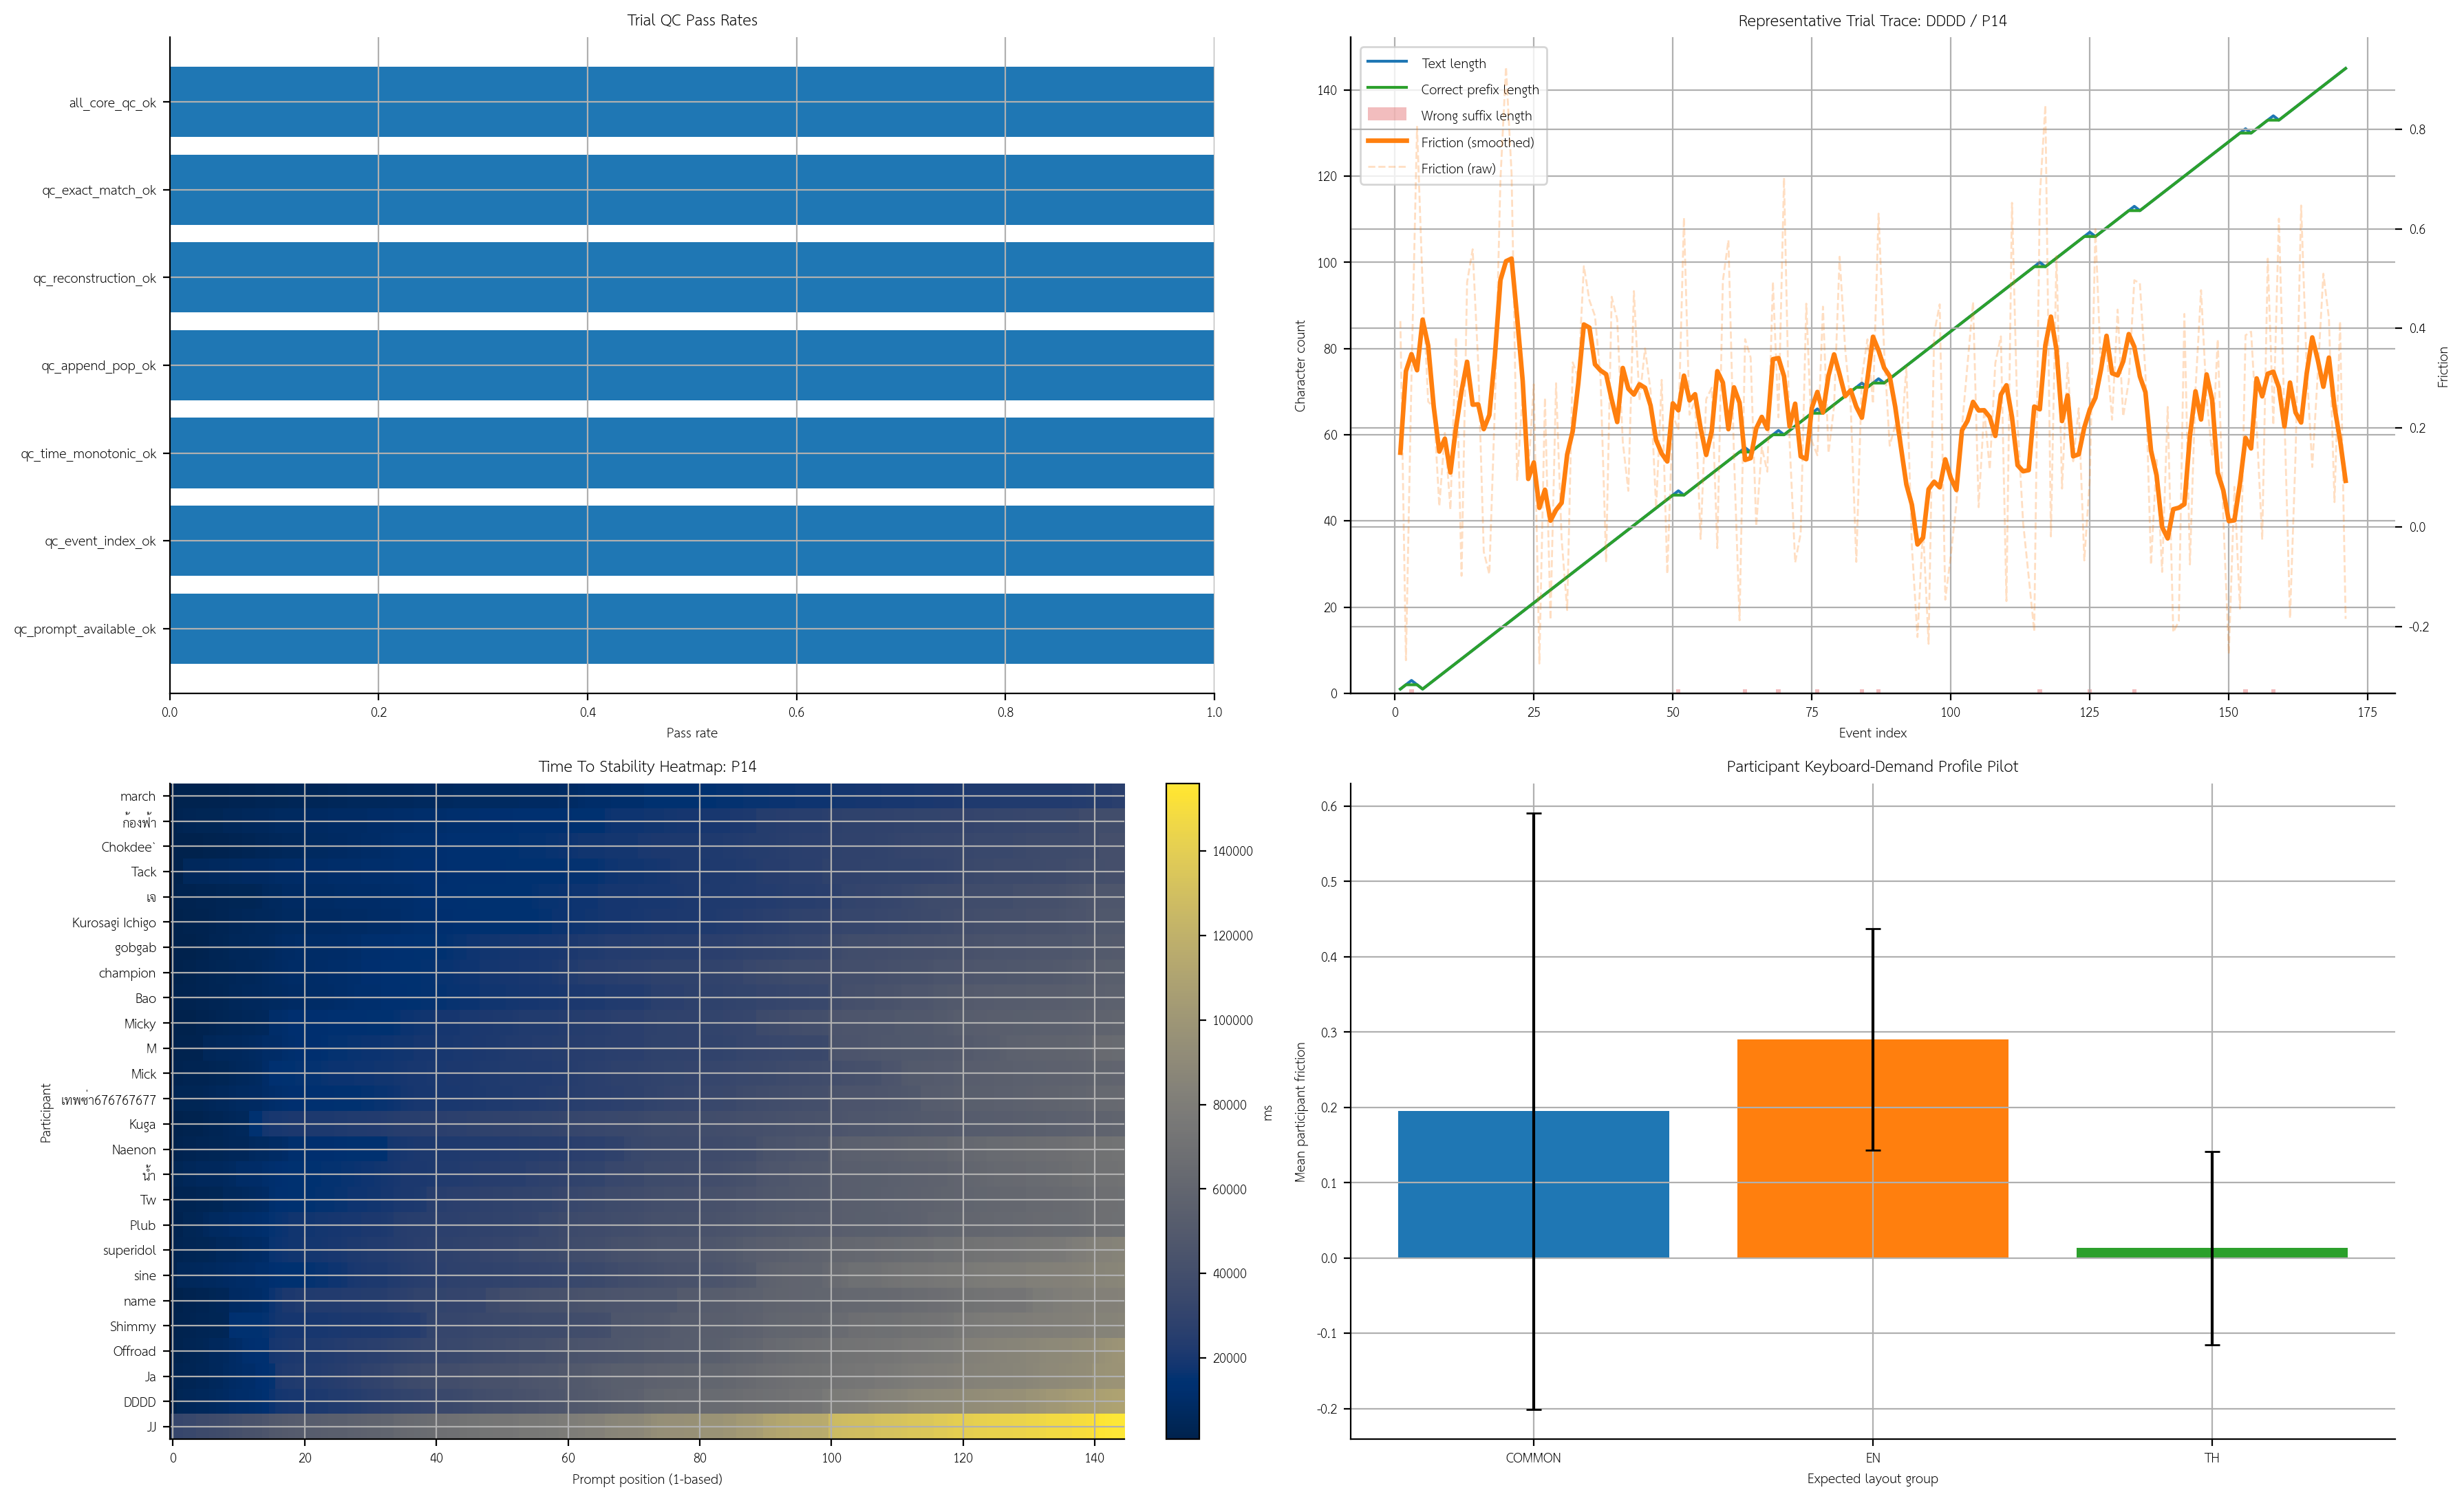
\includegraphics[width=0.96\linewidth]{assets/pilot_trace_P14.png}
  \caption{Object A: pilot event-stream trace for one participant on prompt P14. Each column is one event; the rows show prefix length, wrong-suffix length, and delete flags over time. Spikes in wrong-suffix length mark the onset of error episodes; their subsequent collapse marks backspace-driven recovery.}
  \label{fig:object_a}
\end{figure}

\paragraph{Object B - Scalar friction waveform.}
Object B compresses the multivariate event stream into a single per-event scalar. The friction score weights inter-key timing, delete actions, wrong-suffix depth, planned geometry, and layout switching into one number that rises during struggle and falls during smooth typing. Because all trials are resampled to a fixed length before Euclidean or Matrix Profile comparison, Object~B enables lockstep waveform analysis across participants and prompts. The figure below shows the friction waveform for one participant on P14 alongside its Matrix Profile, where high MP values (discords) flag locally unusual friction shapes.

\begin{figure}[H]
  \centering
  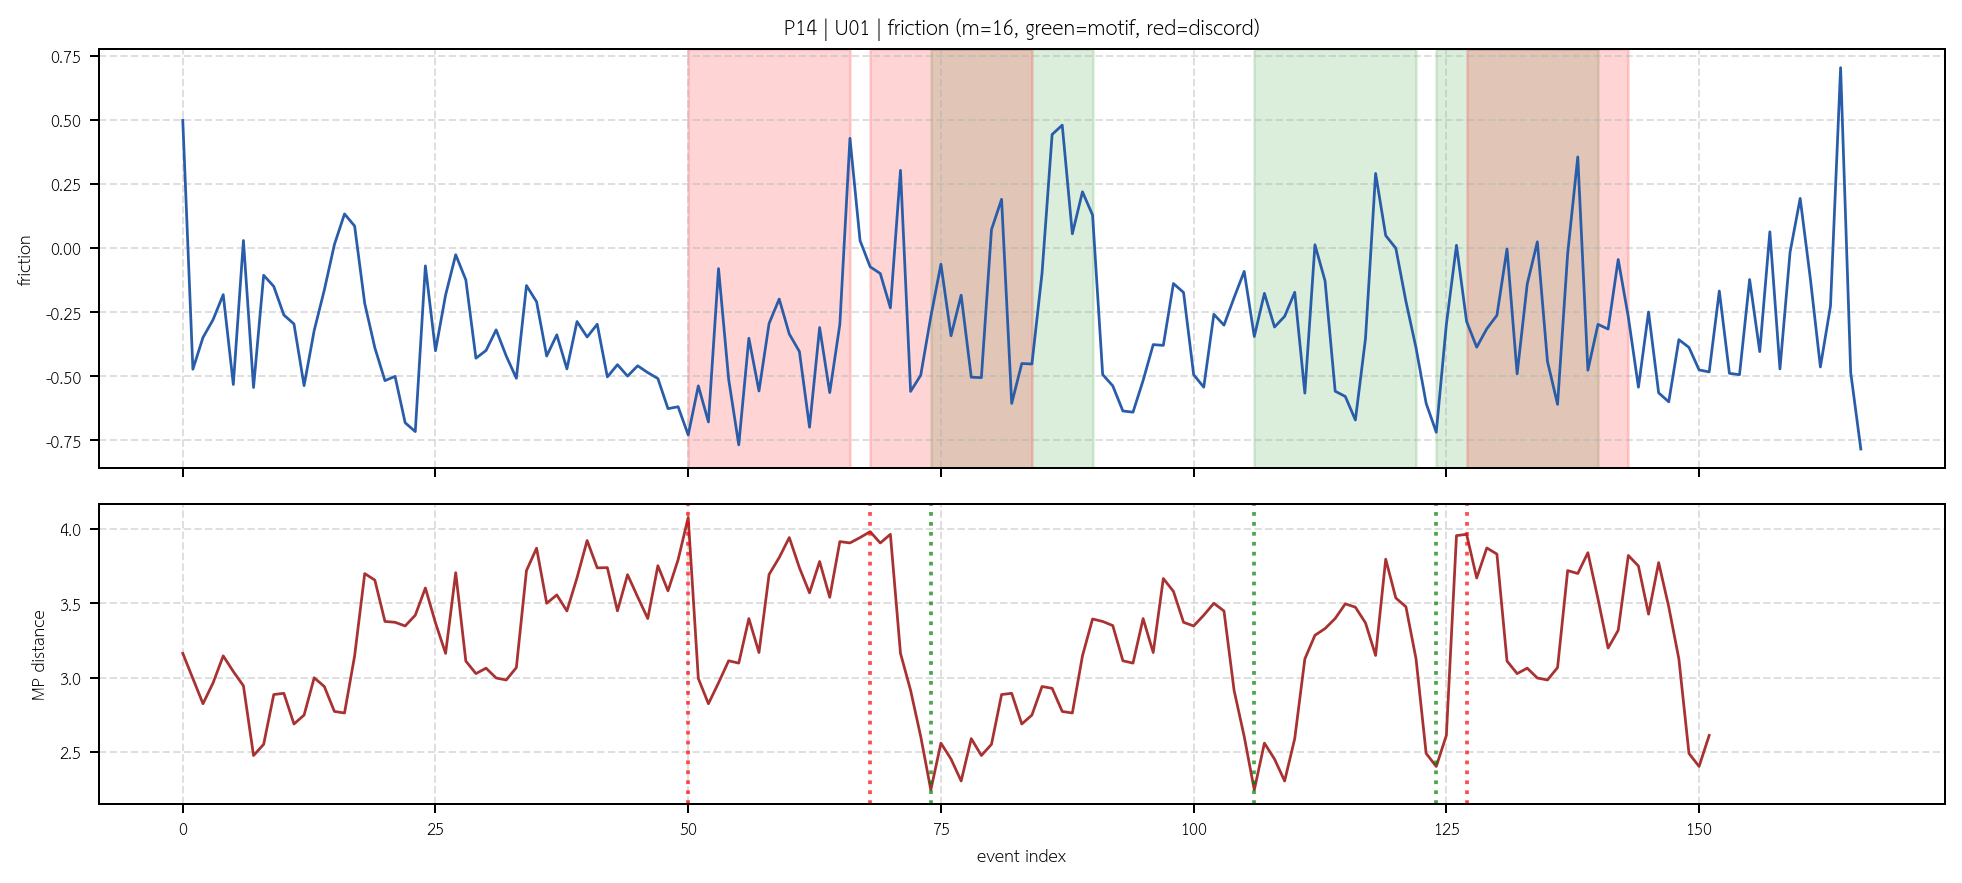
\includegraphics[width=0.96\linewidth]{assets/mp_friction_P14_U01.png}
  \caption{Object B: scalar friction waveform (top) and its Matrix Profile (bottom) for participant U01 on prompt P14. The horizontal axis is event position; the vertical axis of the MP gives the nearest-neighbor distance for each subsequence. High MP values identify segments whose friction shape is unlike any other segment in the trial.}
  \label{fig:object_b}
\end{figure}

\paragraph{Object C - Prompt-position stability sequence.}
Object C shifts the index from event time to prompt character position. For every position in the prompt, it records the median time until that position first becomes stably correct, the wrong-first rate, and the revision count, all aggregated across participants. Object~C has a fixed length equal to the prompt length and is the basis for same-prompt difficulty curves, Euclidean distance heatmaps, and Matrix Profile discord detection on the aggregated difficulty curve. The heatmap below shows \metric{time\_to\_stability\_ms} for all 26 participants across all positions of P14; columns with a warm colour indicate characters where many participants were slow to stabilize.

\begin{figure}[H]
  \centering
  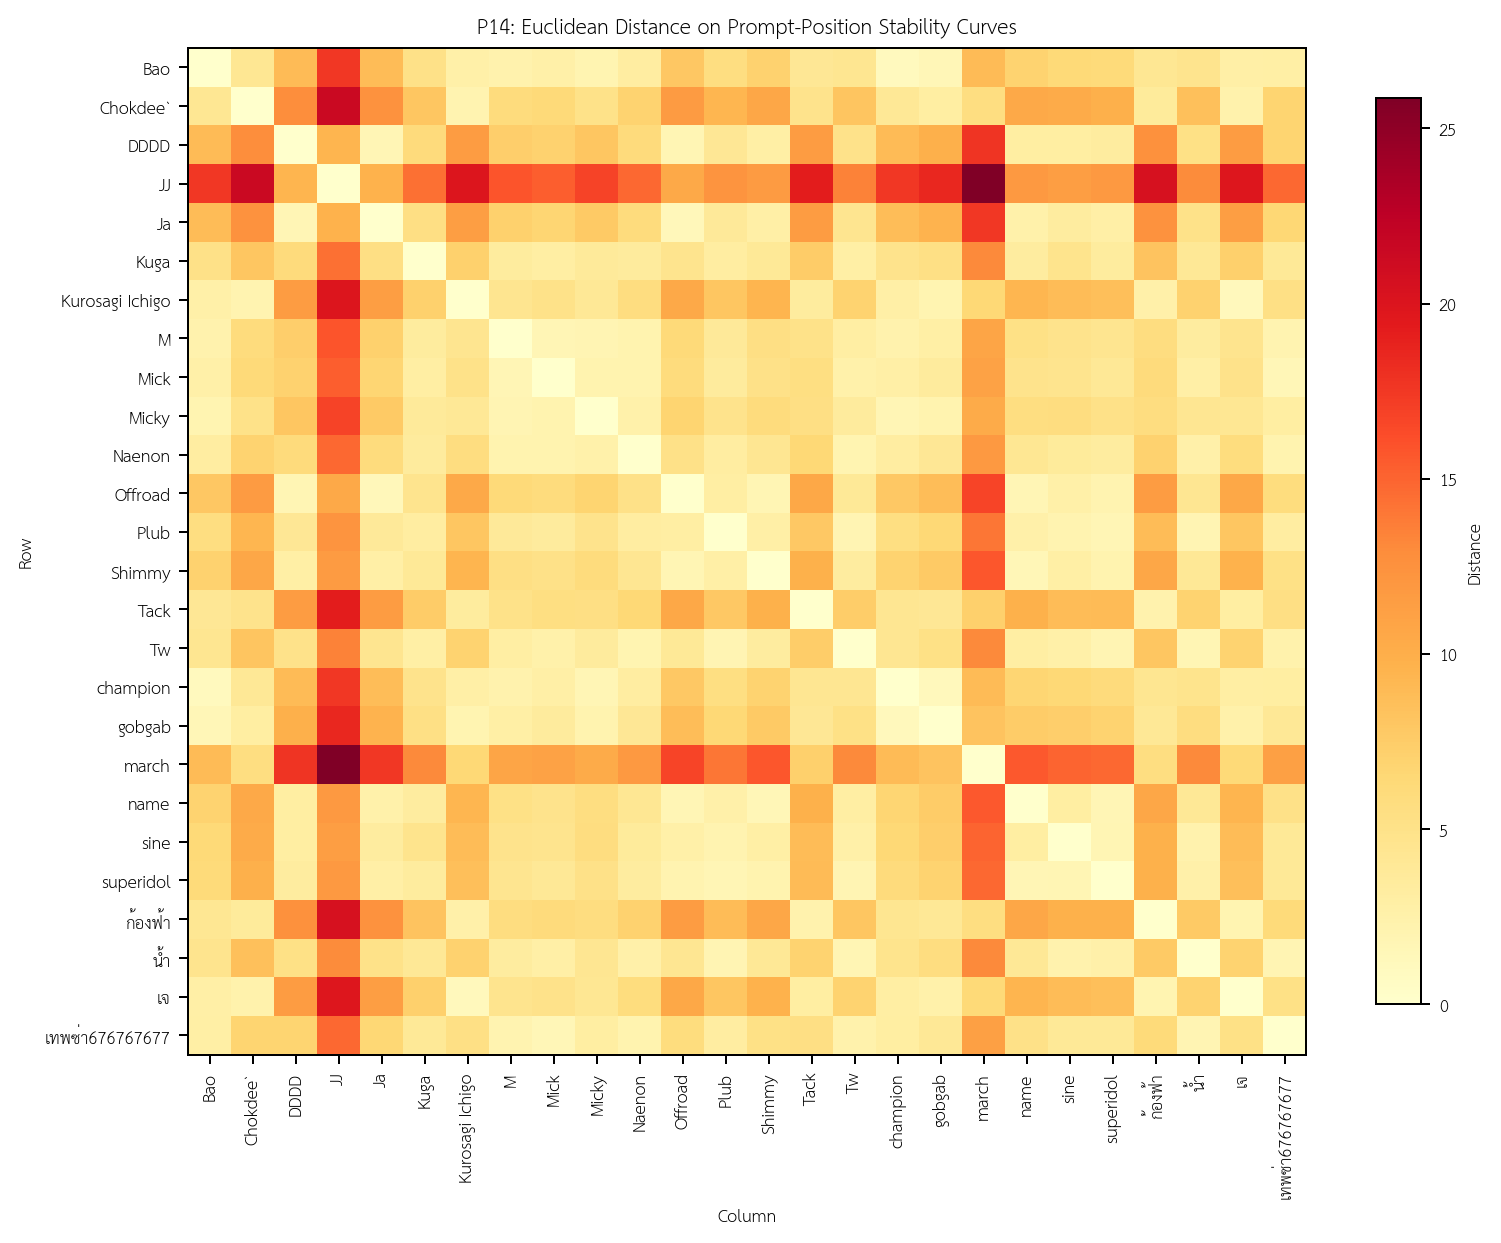
\includegraphics[width=0.98\linewidth]{assets/euclidean_prompt_position_heatmap_P14.png}
  \caption{Object C: prompt-position stability heatmap for P14. Rows are participants (anonymized), columns are prompt positions. Warm colours indicate longer time-to-stability. The spike visible around positions 94–101 corresponds to the Thai numeral ๖ that is the top Matrix Profile discord on this prompt.}
  \label{fig:object_c}
\end{figure}

\paragraph{Object D - Participant keyboard-demand profile.}
Object D aggregates each participant's behavior by keyboard-demand category rather than by prompt position. Each row is one participant; the columns are mean values of \metric{time\_to\_stability\_ms}, \metric{wrong\_first}, and \metric{friction} broken out by character class, shift requirement, layout-switch frequency, and zone. Object~D is a fixed-length feature vector that supports Euclidean participant clustering and comparisons across the cohort. The reordered heatmap below reveals that participants in the fast cluster (U01–U05) have consistently low values across all keyboard-demand columns, while participants in the slow cluster (U24–U26) show elevated values especially in the Thai-numeral and diacritic columns.

\begin{figure}[H]
  \centering
  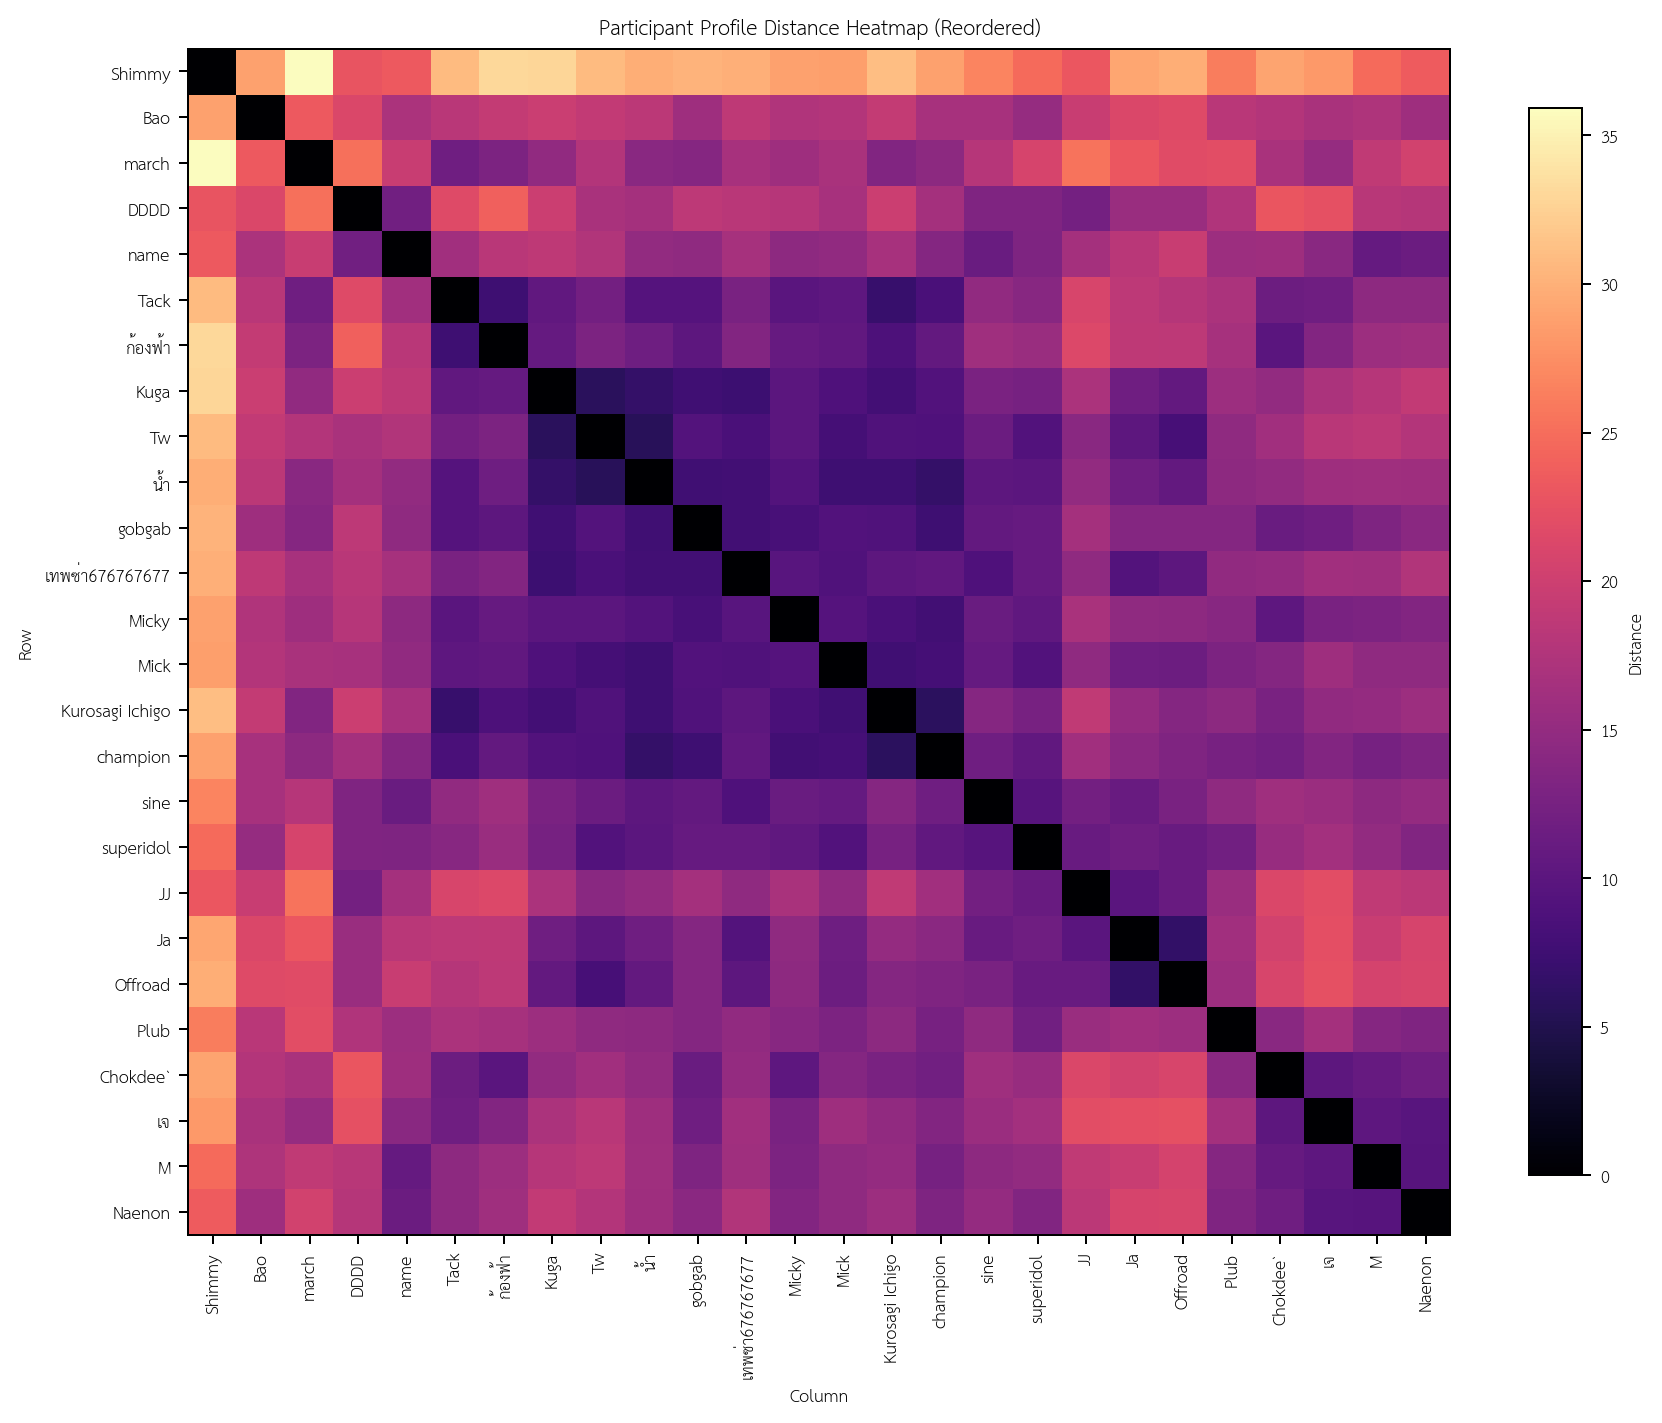
\includegraphics[width=0.96\linewidth]{assets/participant_profile_euclidean_heatmap_reordered.png}
  \caption{Object D: participant keyboard-demand profile heatmap, rows reordered by hierarchical cluster. Each column is one keyboard-demand feature averaged across all trials for that participant. Cluster structure is clearest in the Thai-numeral and layout-switch columns.}
  \label{fig:object_d}
\end{figure}

\begin{thebibliography}{9}

\bibitem{berndt1994dtw}
D. J. Berndt and J. Clifford.
\newblock Using Dynamic Time Warping to Find Patterns in Time Series.
\newblock \emph{Proceedings of the AAAI-94 Workshop on Knowledge Discovery in Databases}, 1994.
\newblock \url{https://ed.aaai.org/Library/Workshops/1994/ws94-03-031.php}

\bibitem{yeh2016matrixprofile}
C.-C. M. Yeh, Y. Zhu, L. Ulanova, N. Begum, Y. Ding, H. A. Dau, D. F. Silva, A. Mueen, and E. Keogh.
\newblock Matrix Profile I: All Pairs Similarity Joins for Time Series: A Unifying View That Includes Motifs, Discords and Shapelets.
\newblock \emph{IEEE ICDM}, 2016.
\newblock \url{https://ieeexplore.ieee.org/document/7837992}

\bibitem{law2019stumpy}
S. M. Law.
\newblock STUMPY: A Powerful and Scalable Python Library for Time Series Data Mining.
\newblock \emph{Journal of Open Source Software}, 4(39), 1504, 2019.
\newblock \url{https://joss.theoj.org/papers/10.21105/joss.01504}

\bibitem{floyd1962}
R. W. Floyd.
\newblock Algorithm 97: Shortest Path.
\newblock \emph{Communications of the ACM}, 5(6), 345, 1962.

\bibitem{warshall1962}
S. Warshall.
\newblock A Theorem on Boolean Matrices.
\newblock \emph{Journal of the ACM}, 9(1), 11-12, 1962.
\newblock \url{https://projects.csail.mit.edu/jacm/References/warshall1962%3A11.html}

\end{thebibliography}

\end{document}
